\section{Beta Ablation Study}\label{sec:ablation_beta}

We consider the effect of the $\beta$ hyperparameter of \method{} introduced in Section \ref{dpaf}, controlling the speed of the prior decay. To show the effect of this hyperparameter, we display the performance of \method for the toy and surrogate-based benchmarks across all prior qualities. 
We emphasize the trade-off between high-end performance on good priors and robustness to bad priors. In general, a higher value of $\beta$ yields better performance for good priors, but makes \method slower to recover from bad priors. This behaviour follows intuition and the results provided in Section~\ref{sec:theory}. 

In Figure \ref{fig:beta_sens}, we display how \method performs for different choices of $\beta$, and once again provide sampling from the prior and Spearmint as baselines. Following the prior decay parameter baseline by~\citep{souza2021bayesian}, we show that the choice of $\beta=10$ onsistently gives one of the best performances for strong priors, while retaining good overall robustness. Nearly all choices of $\beta$ give a final performance better than that of Spearmint for good priors. Additionally, there is a clear relationship between final performance and $\beta$ on all good priors. This is best visualized in the weak XGBoost experiment, where the final performances are distinctly sorted by increasing $\beta$. Similar patterns are not as apparent in the final performance on wrong priors. This behaviour highlights the benefits of slowly decaying the prior. Overall, \method is competitive for a wide range of $\beta$, but suffers slightly worse final performance on good priors for low values of $\beta$.
\begin{figure}[!b]
    \centering
    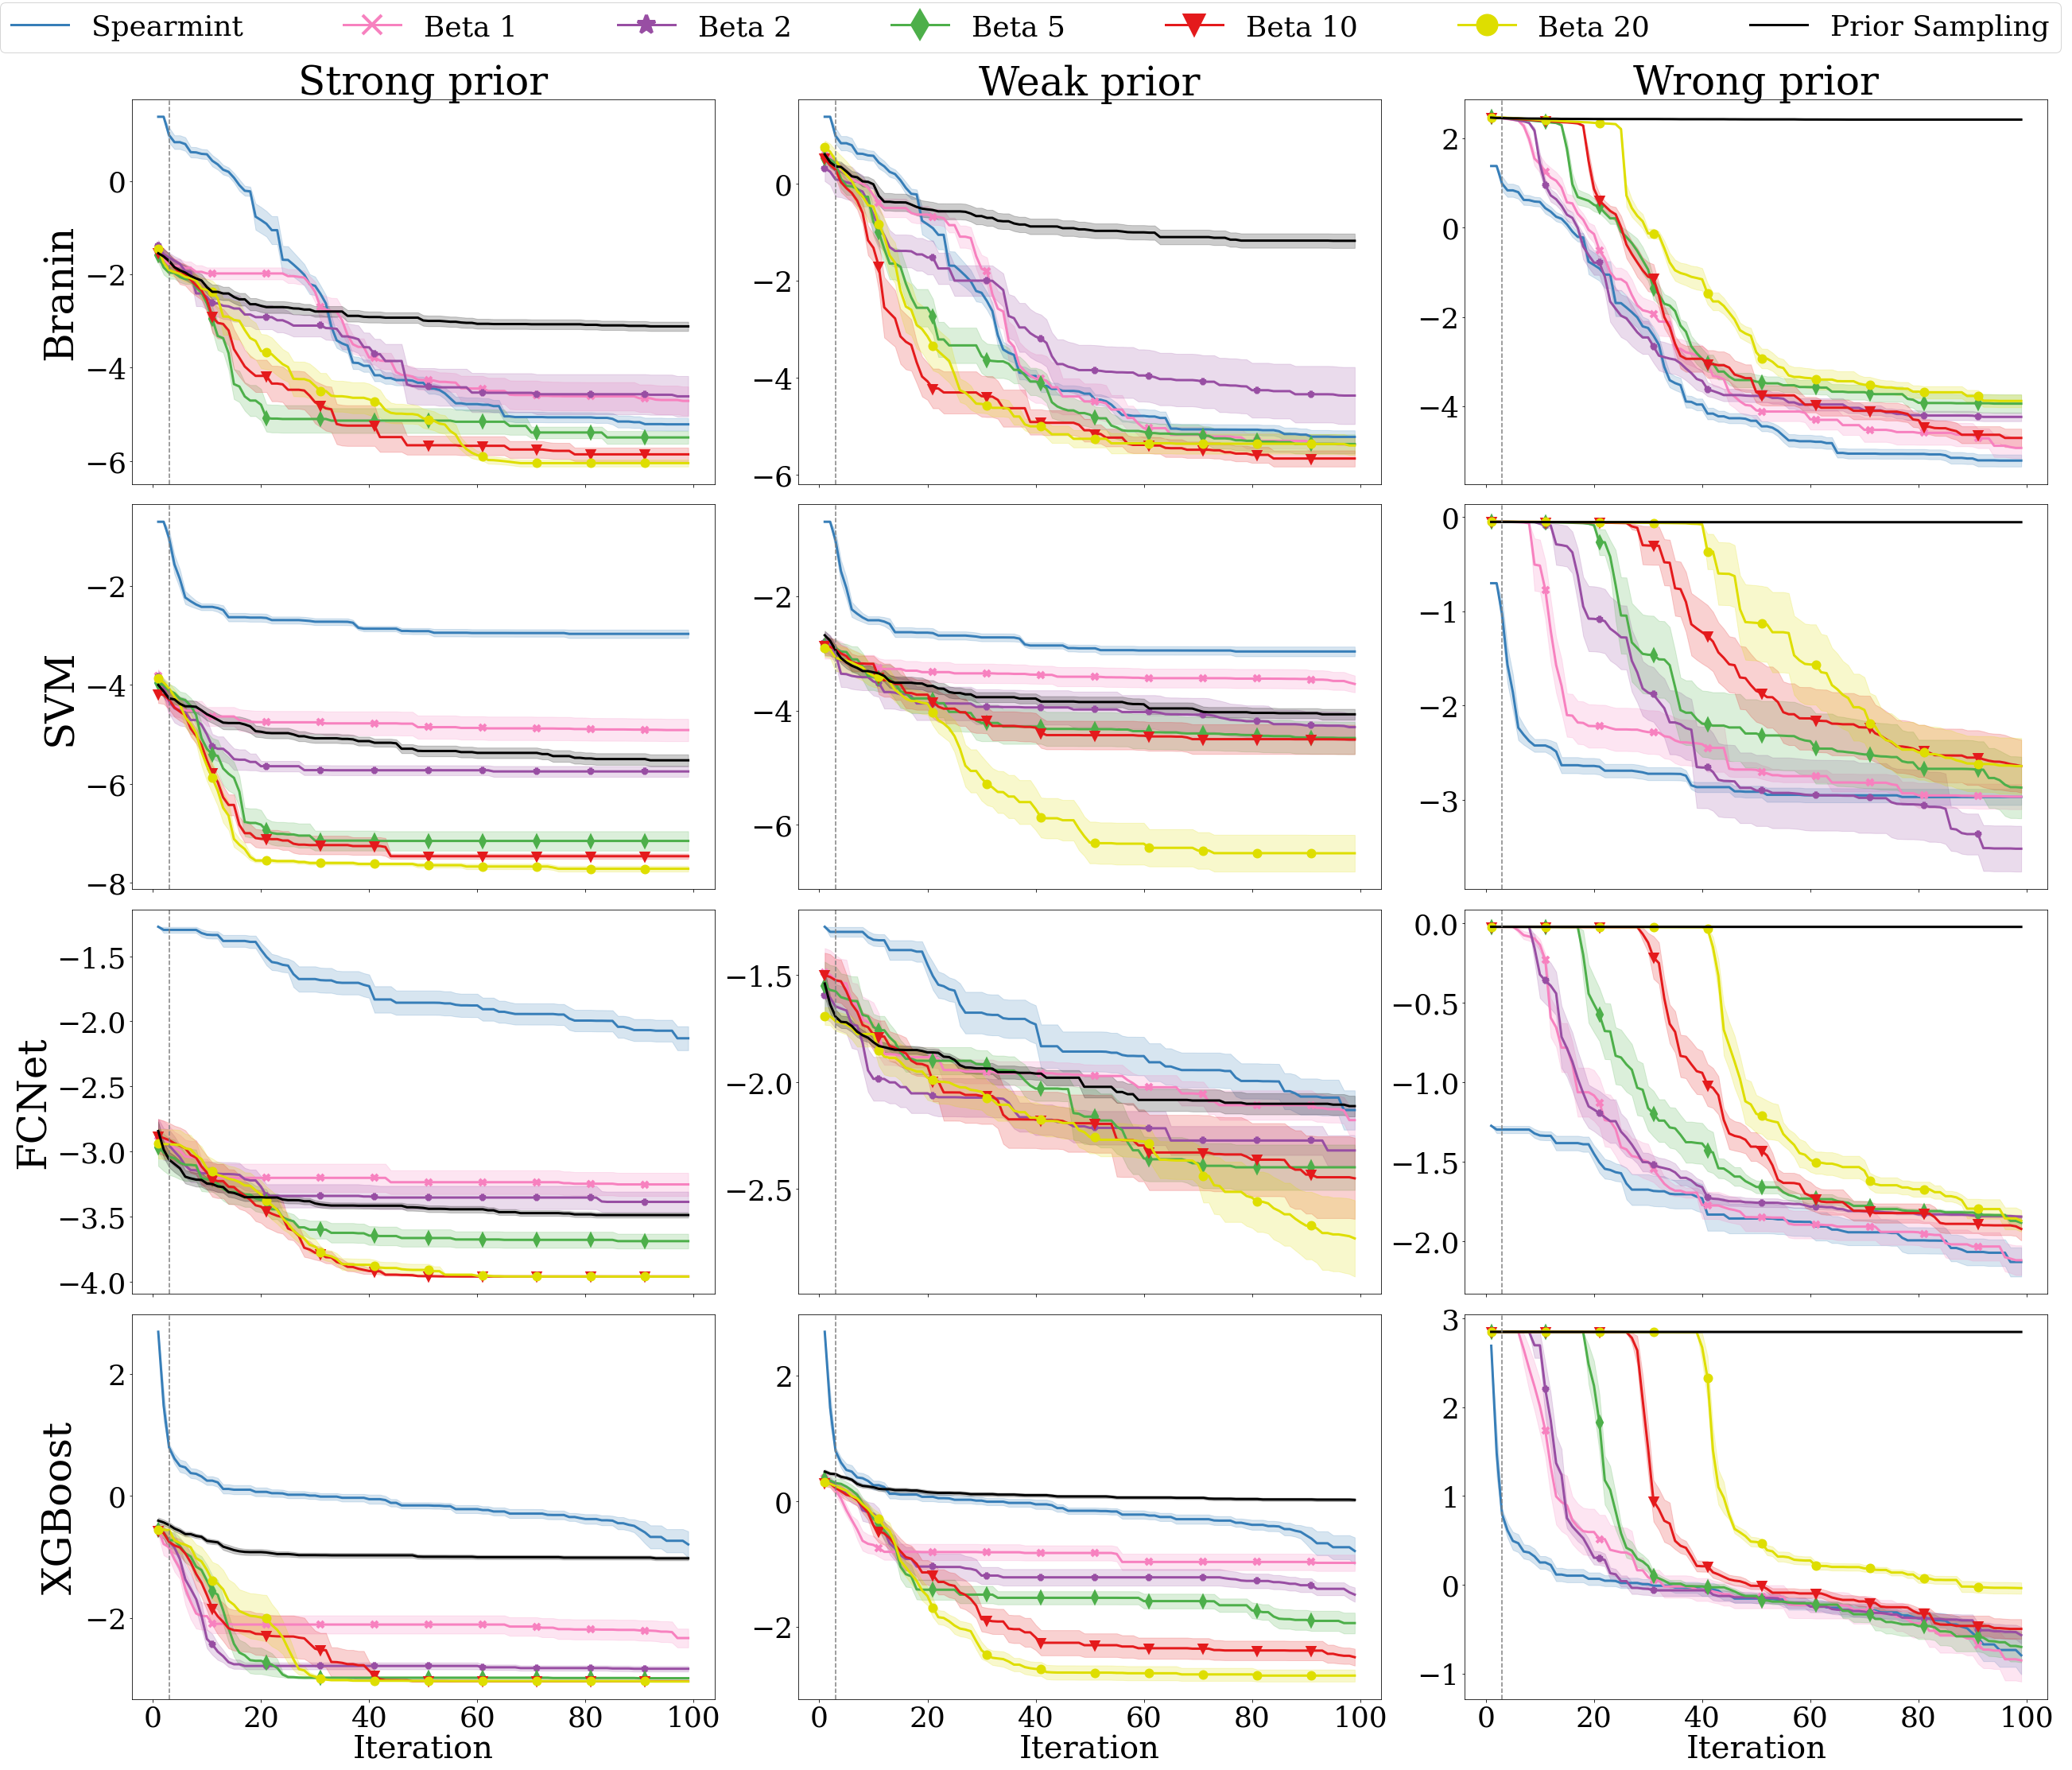
\includegraphics[width=\linewidth]{images/all_betas.png}[h]
    \caption{Comparison of \method and Spearmint with varying values of $\beta$ for Branin and Profet benchmarks for the strong, weak and wrong prior qualities. The mean and standard error of log simple regret is displayed over 100 iterations, averaged over 10 repetitions. Iteration 1 is removed for visibility purposes. The vertical line represents the end of the initial design phase.}
    \label{fig:beta_sens}
\end{figure}

%\luigi{This introductory paragraph needs to be adapted to the new flow in appendix B, which includes new sections (PI, etc.).}
\section{\method Versatility} \label{sec:other_fw}
We show the versatility of \method by implementing it in numerous variants of SMAC~\cite{smac}, a well-established HPO framework which supports both GP and RF surrogates, and a majority of the myopic acquisition functions mentioned in Section \ref{sec:background}. We showcase the performance of \method{}-EI, \method{}-PI, \method{}-UCB and \method{}-TS on the general formulation of \method{} with a GP surrogate, as well as \method{}-EI with an RF surrogate, which requires a minor adaptation. 
\begin{figure}[tb]
    \centering
    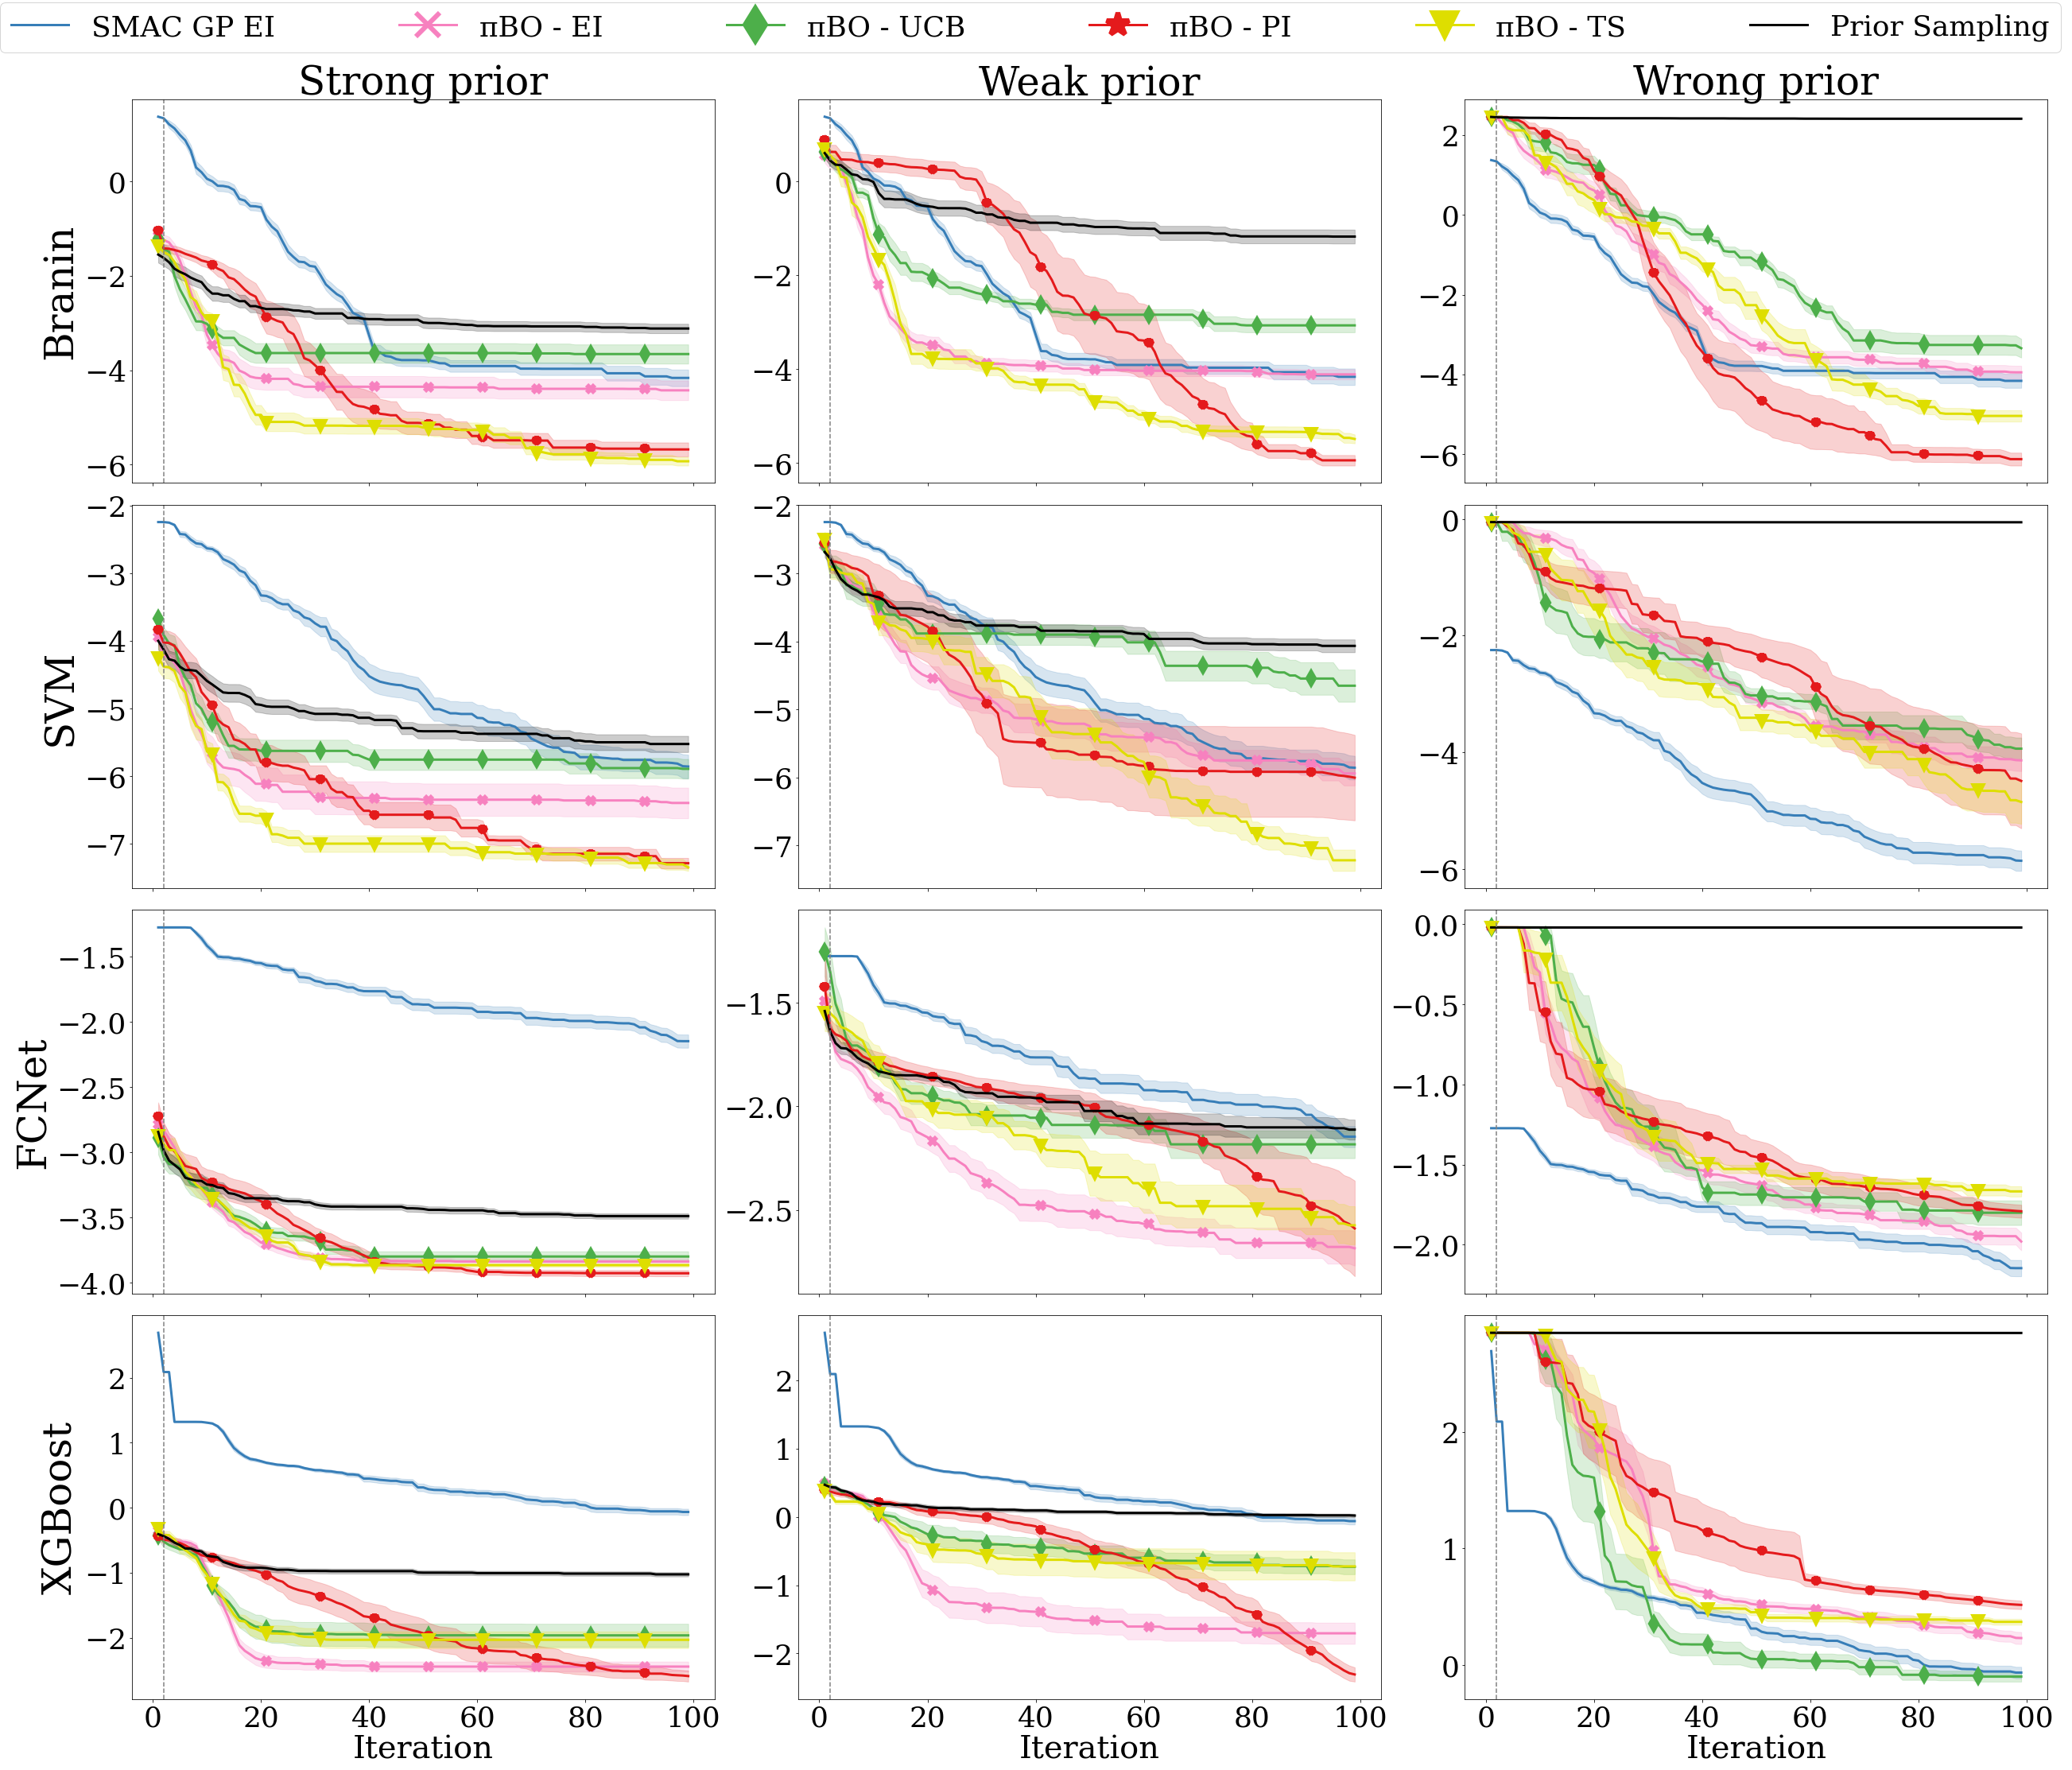
\includegraphics[width=\linewidth]{images/all_acqs.png}
    \caption{\method{} on SMAC using a GP surrogate for the EI, UCB, PI and TS acquisition functions, $\beta=10$ for Branin and Profet benchmarks for varying prior qualities. The mean and standard error of log simple regret is displayed over 100 iterations, averaged over 10 repetitions. Iteration 1 is removed for visibility purposes. The vertical line represents the end of the initial design phase.}
    \label{fig:acq_results}
\end{figure}
\begin{figure}[tb]
    \centering
    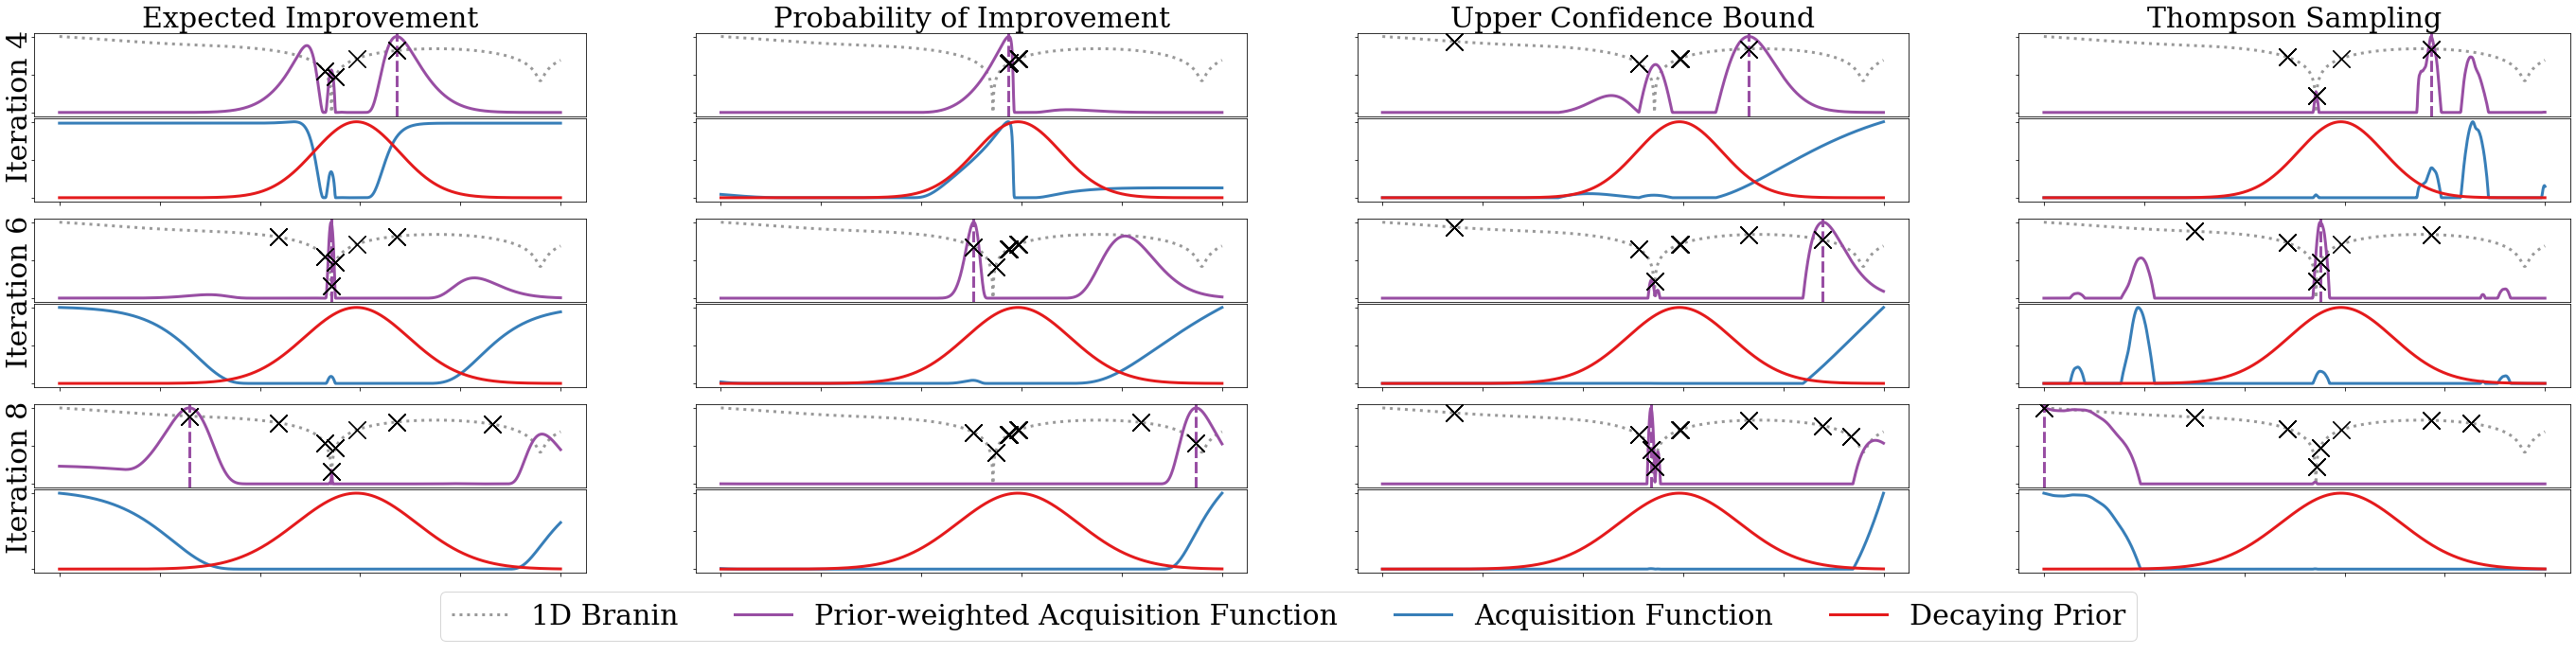
\includegraphics[width=\linewidth]{images/all_acqs_behaviour.png}
    \caption{Point selection strategy evolution for \method on SMAC with a GP surrogate for the EI, PI, UCB and TS acquisition functions on the Log-1D-Branin function. The plots show rescaled values of the prior-weighted acquisition function (purple), the regular acquisition function (blue) and $\pi_n$ (red) on a 1D-Branin (grey) with global optimum in the center of the search space and the current selection as a vertical violet line. The rows represent iterations 4, 6 and 8 for a run with $\beta=2$. }
    \label{fig:acq_behaviour}
\end{figure}

\subsection{General formulation of \method{}}
To allow for the universality of \method{} across several acquisition function, we must consider the various magnitudes of acquisition functions. As UCB and TS typically output values in the same order of magnitude and sign as the objective function, we do not want the behaviour of \method to be affected by such variations. 

The solution to the problem referenced above is to add a simple affine transformation to the observations, $\{y_i\}_{i=1}^n$, by subtracting by the incumbent, $y^*_n$. As such, we consider at each time step not the original dataset, $\mathcal{D}_n = \{{(\bm{x}_i, y_i)}\}_{i=1}^n$, but the augmented dataset $\hat{\mathcal{D}}_n = \{{(\bm{x}_i, y_i-y^*_n)}\}_{i=1}^n$. With this formulation, we get the desired scale- and sign-invariance in the UCB and TS acquisition functions, without changing the original strategy of any of the acquisition function. Notably, this change leaves prior-weighted EI and PI unaffected.

\subsection{Random Forest Surrogate}\label{ref:rf_surr}
We now demonstrate \method{} with a RF surrogate model. In the SMAC implementation of the RF surrogate, the model forms piece-wise constant mean and covariance functions. 
Naturally, this leads to the EI, PI or UCB acquisition function surface being piece-wise constant as well. Consequently, an acquisition function with a RF surrogate will typically have a region of global optima. The choice of the next design point is then selected uniformly at random among the candidate optima. We wish to retain this randomness when applying \method. As such, we require the prior to be piece-wise constant, too. 
%\begin{figure}[tb]
%    \centering
%    
\includegraphics[width=\linewidth]{images/smac_rf_broken.png}
%    \caption{\method{}-SMAC-RF using Expected Improvement: Comparison of \method on Spearmint %(EI) and SMAC (EI) using a RF surrogate, $\beta=10$, and the supporting frameworks for Branin %and Profet benchmarks for varying prior qualities. The mean and standard error of log simple %regret is displayed over 100 iterations, averaged over 10 repetitions. Iteration 1 is removed %for visibility purposes. The vertical line represents the end of the initial design phase.}
%    \label{fig:smac_rf_broken}
%\end{figure}
%Since \method allows for any prior distribution to be used in optimization, we must ensure that the prior-weighted acquisition function is piece-wise constant for any prior when a RF surrogate is used. 
To do so, we employ a binning approach, that linearly rounds prior values after applying the decay term. The granularity of the binning decreases at the same rate as the prior, allowing the piece-wise constant regions of the prior grow in size as optimization progresses. In Figure~\ref{fig:smac_rf_behaviour}, we demonstrate the importance of the piece-wise constant acquisition function by showing the point selection when applying a \method with a continuous prior to an RF surrogate (left) and when applying the binning approach (right). Notably, the smooth prior on the left repeatedly proposes design points very close to previous points, as the prior forces the selection of points near the boundary of a promising region. Thus, the surrogate model rarely improves, and the optimization gets stuck at said boundary for multiple iterations at a time. This is best visualized at iteration 5 and 10, where similar points have been selected for all iterations in the time span. With the binned prior on the right, the selection of design points occurs randomly within a region, avoiding the static point selection and updating of non-modified approach.
\begin{figure}[tb]
    \centering
    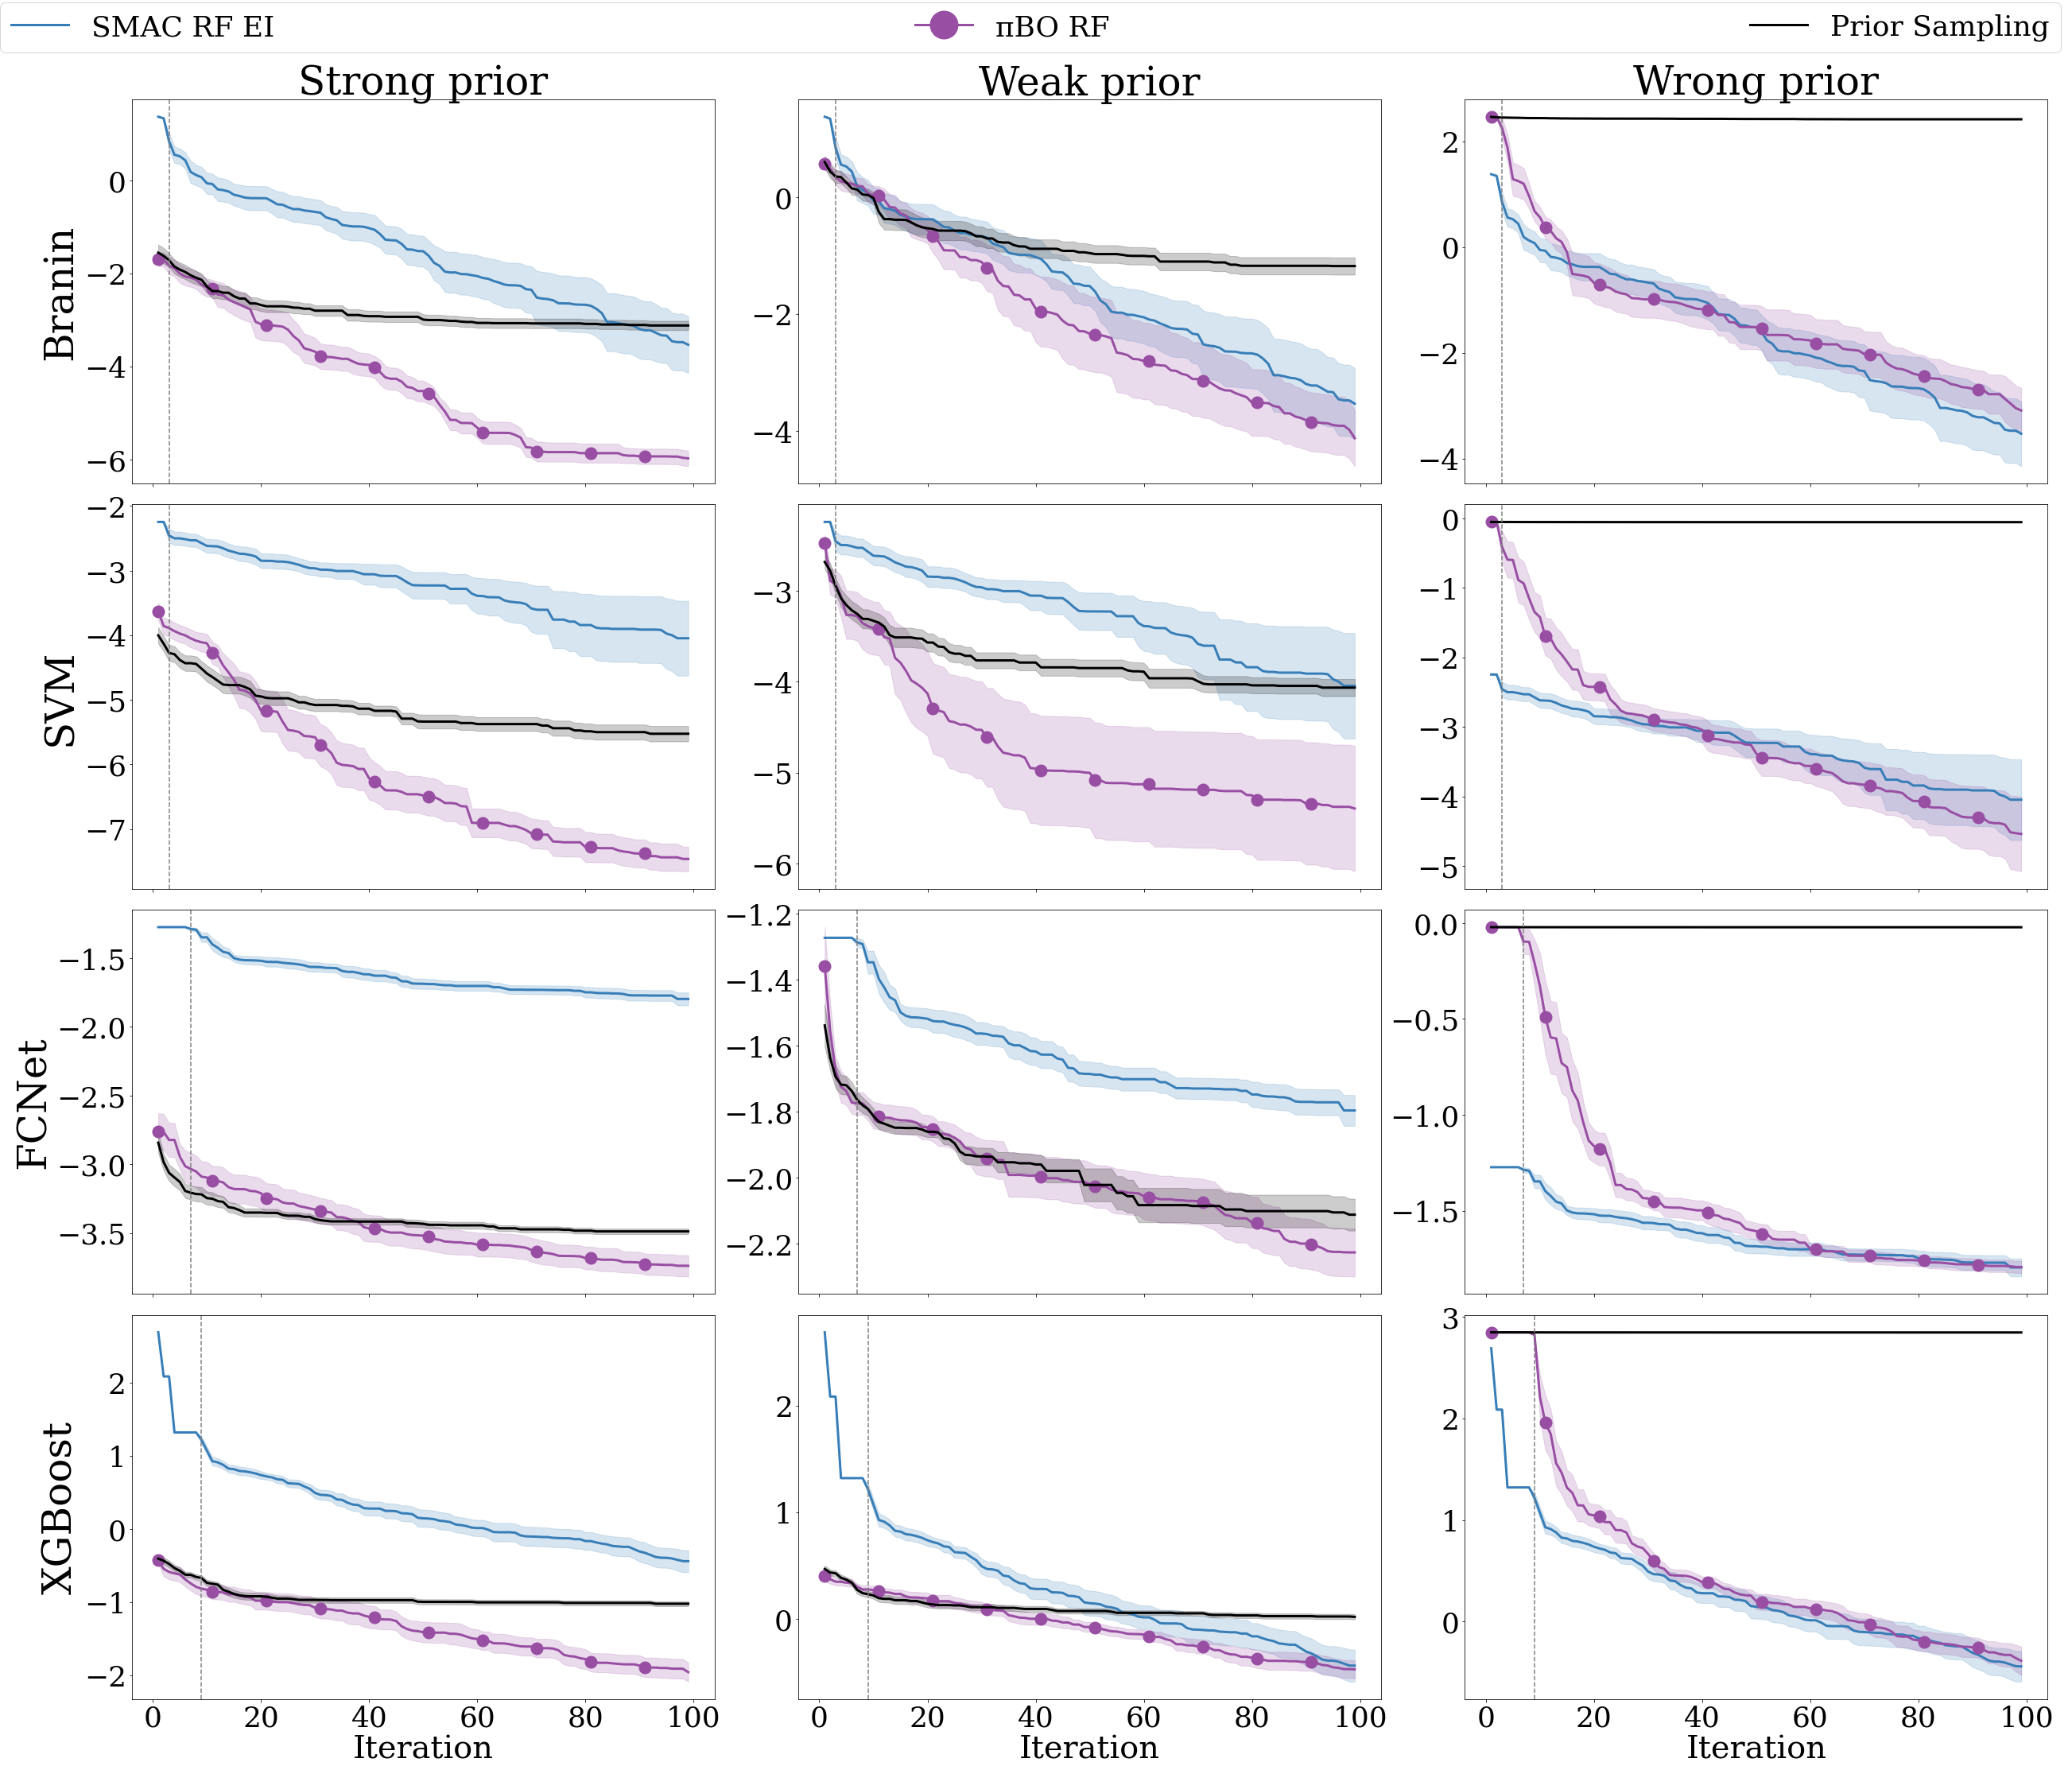
\includegraphics[width=\linewidth]{images/rf_results.png}
    \caption{\method{} with binning and SMAC using and RF surrogate and EI acquisition function, $\beta=10$, and the supporting frameworks for Branin and Profet benchmarks for varying prior qualities. The mean and standard error of log simple regret is displayed over 100 iterations, averaged over 10 repetitions. Iteration 1 is removed for visibility purposes. The vertical line represents the end of the initial design phase.}
    \label{fig:rf_results}
\end{figure}
\begin{figure}[tb]
    \centering
    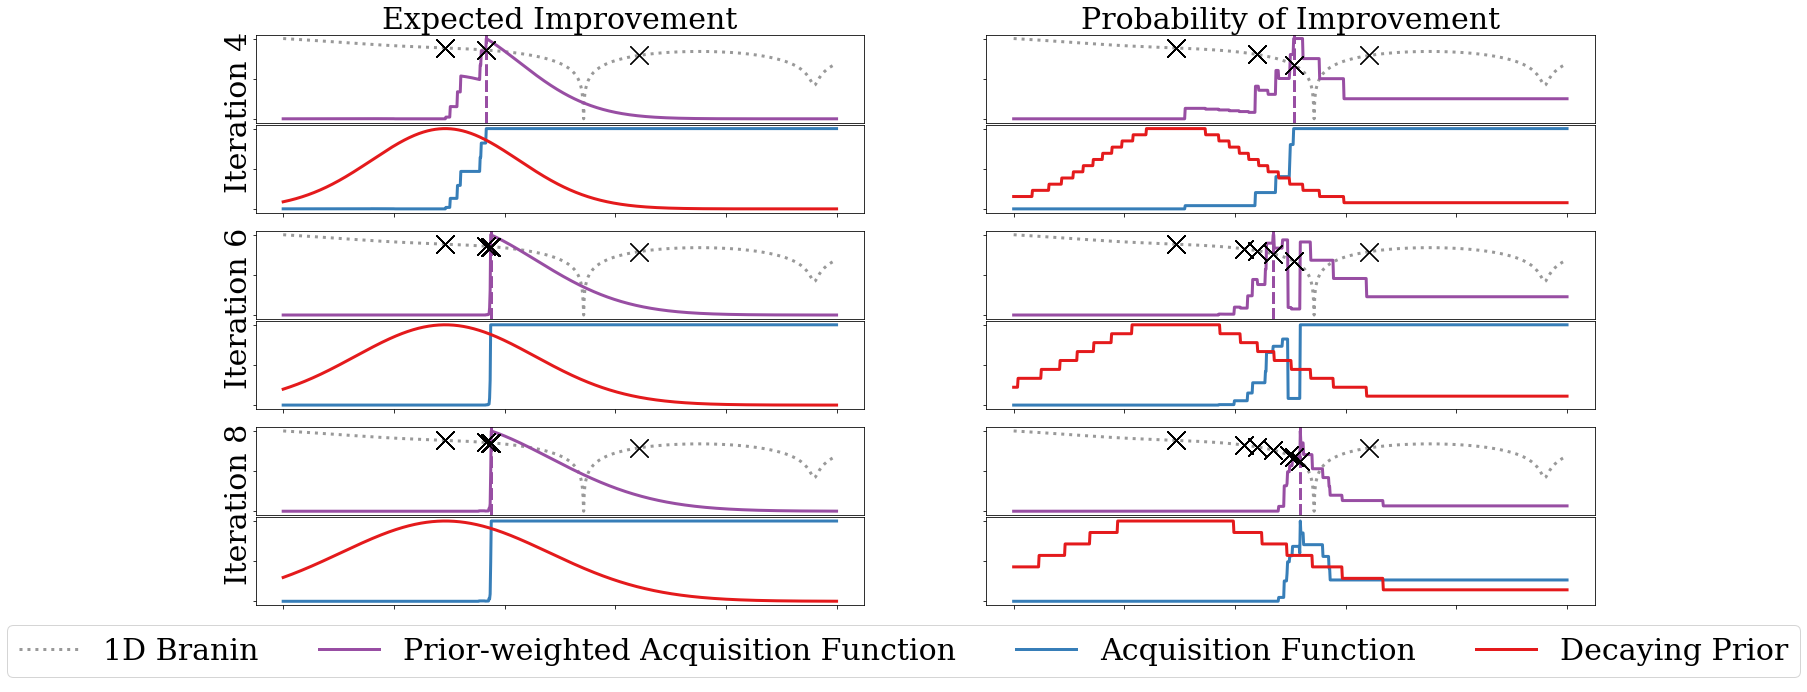
\includegraphics[width=\linewidth]{images/rf_binned_prior.png}
    \caption{Point selection strategy evolution for \method on SMAC with a RF surrogate, when employing a smooth prior (left) and binned prior (right) for the 1D-Branin function. The plots show rescaled values of prior-weighted EI (purple), EI (blue) and $\pi_n$ (red) on a 1D-Branin (grey) with global optimum in the center of the search space and the current selection as a vertical violet line. The rows represent iterations 5, 10, 15 and 20, for a run with $\beta=5$. }
    \label{fig:smac_rf_behaviour}
\end{figure}
In Figure~\ref{fig:rf_results}, we report the performance of \method with a RF surrogate and the binning approach. This approach is competitive, as it provides substantial improvement over SMAC, improves over sampling from the prior, and quickly recovers from misleading priors. Notably, the binning is not required for discrete parameters, as the piece-wise constant property holds by default. Thus, this adaptation is only necessary for continuous parameters.

\section{Other Prior-based Approaches} \label{sec:competition}
We now demonstrate the performance of \method{} for five different functions and HPO Surrogates: Branin, Hartmann-6, as well as three tasks from the Profet suite - SVM, FCNet and XGBoost. We compare all frameworks for priors over the optimum - namely BOPrO~\cite{souza2021bayesian}, BOWS~\cite{RAMACHANDRAN2020105663}, TPE~\cite{bergstra-nips11a}, PS-G~\cite{Li2020IncorporatingEP}. The performance of \method{} is shown on two different frameworks - Spearmint and Hypermapper - to allow for fair comparison and display cross-framework consistency. As BOWS is implemented in Spearmint and BOPrO in Hypermapper, they appear in the plots retaining to their framework. We display each approach with vanilla Spearmint/Hypermapper, with normal initialization, as an additional baseline. Moreover, we display the performance of \method implemented in Spearmint, as well as Mode + Spearmint, on the MLP tuning tasks.

\begin{figure}
    \centering
    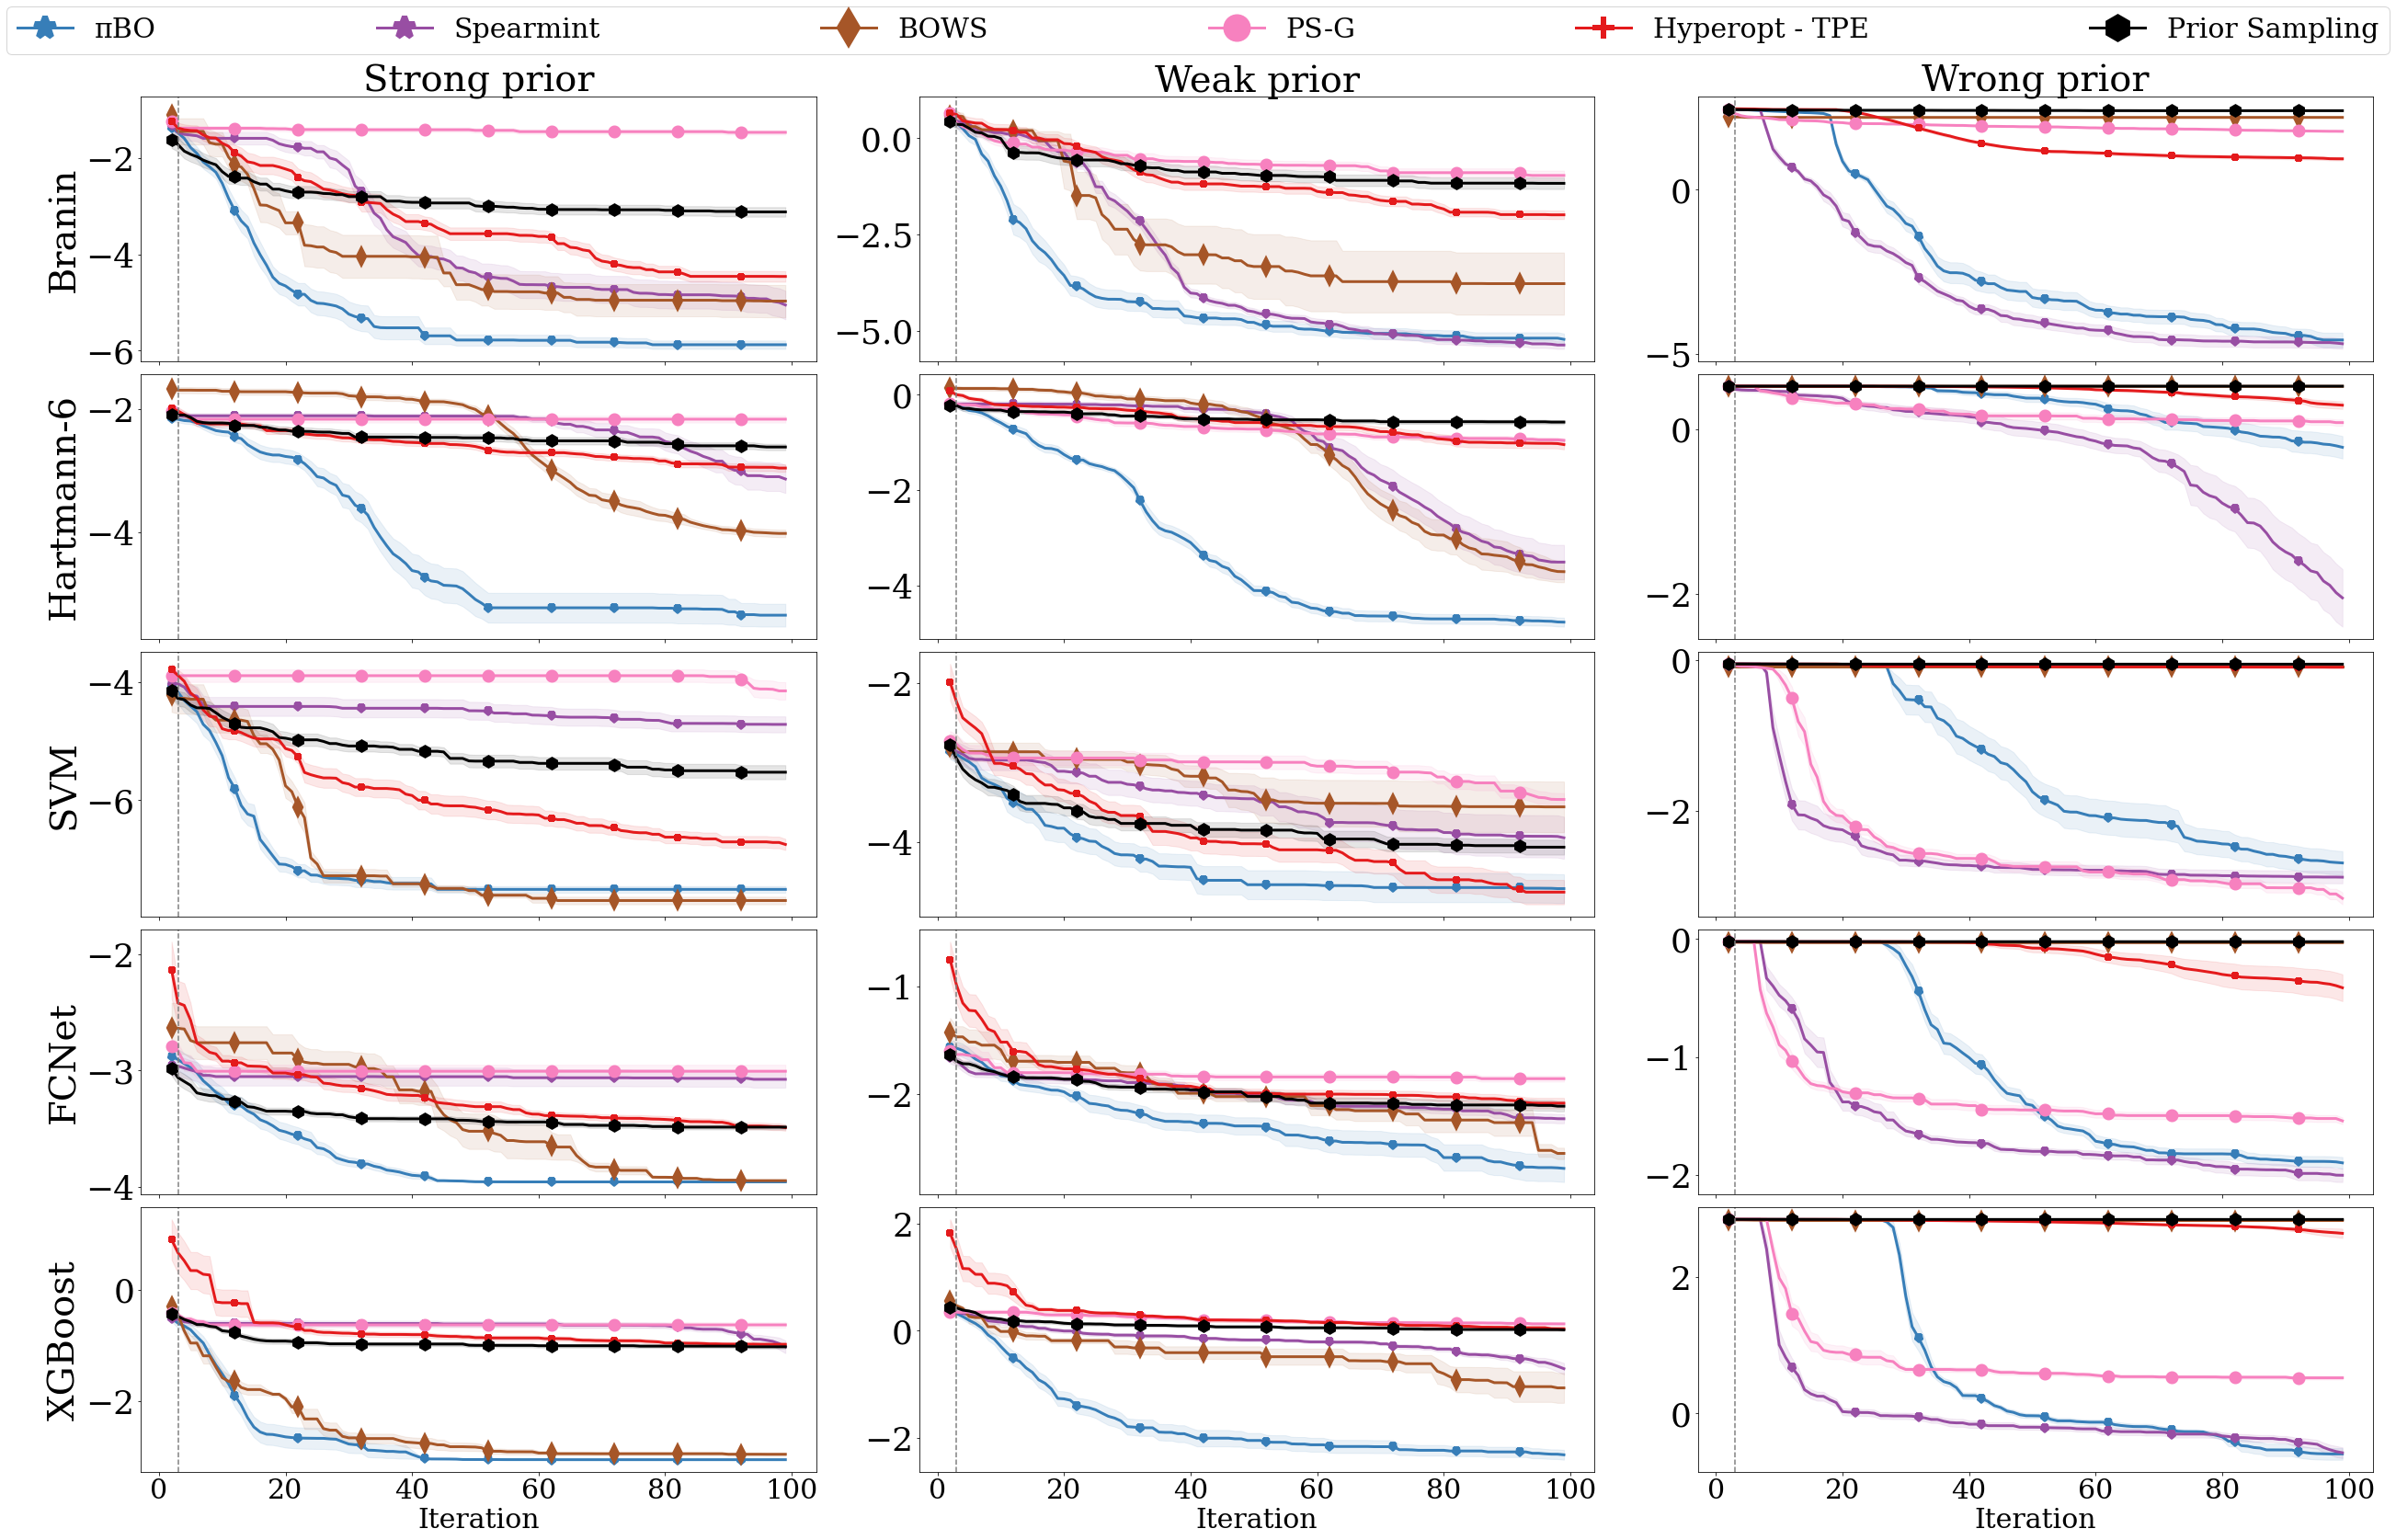
\includegraphics[width=\linewidth]{images/profet_spearmint.png}
    \caption{Comparison of \method{}, Spearmint and other approaches for priors over the optimum for Branin, Hartmann and Profet benchmarks. \method{} is implemented in Spearmint. The mean and standard error of log simple regret is displayed over 100 iterations, averaged over 20 repetitions. Iteration 1 is removed for visibility purposes. The vertical line represents the end of the initial design phase.}
    \label{fig:appendix_spearmint}
\end{figure}


\begin{figure}[h]
    \centering
    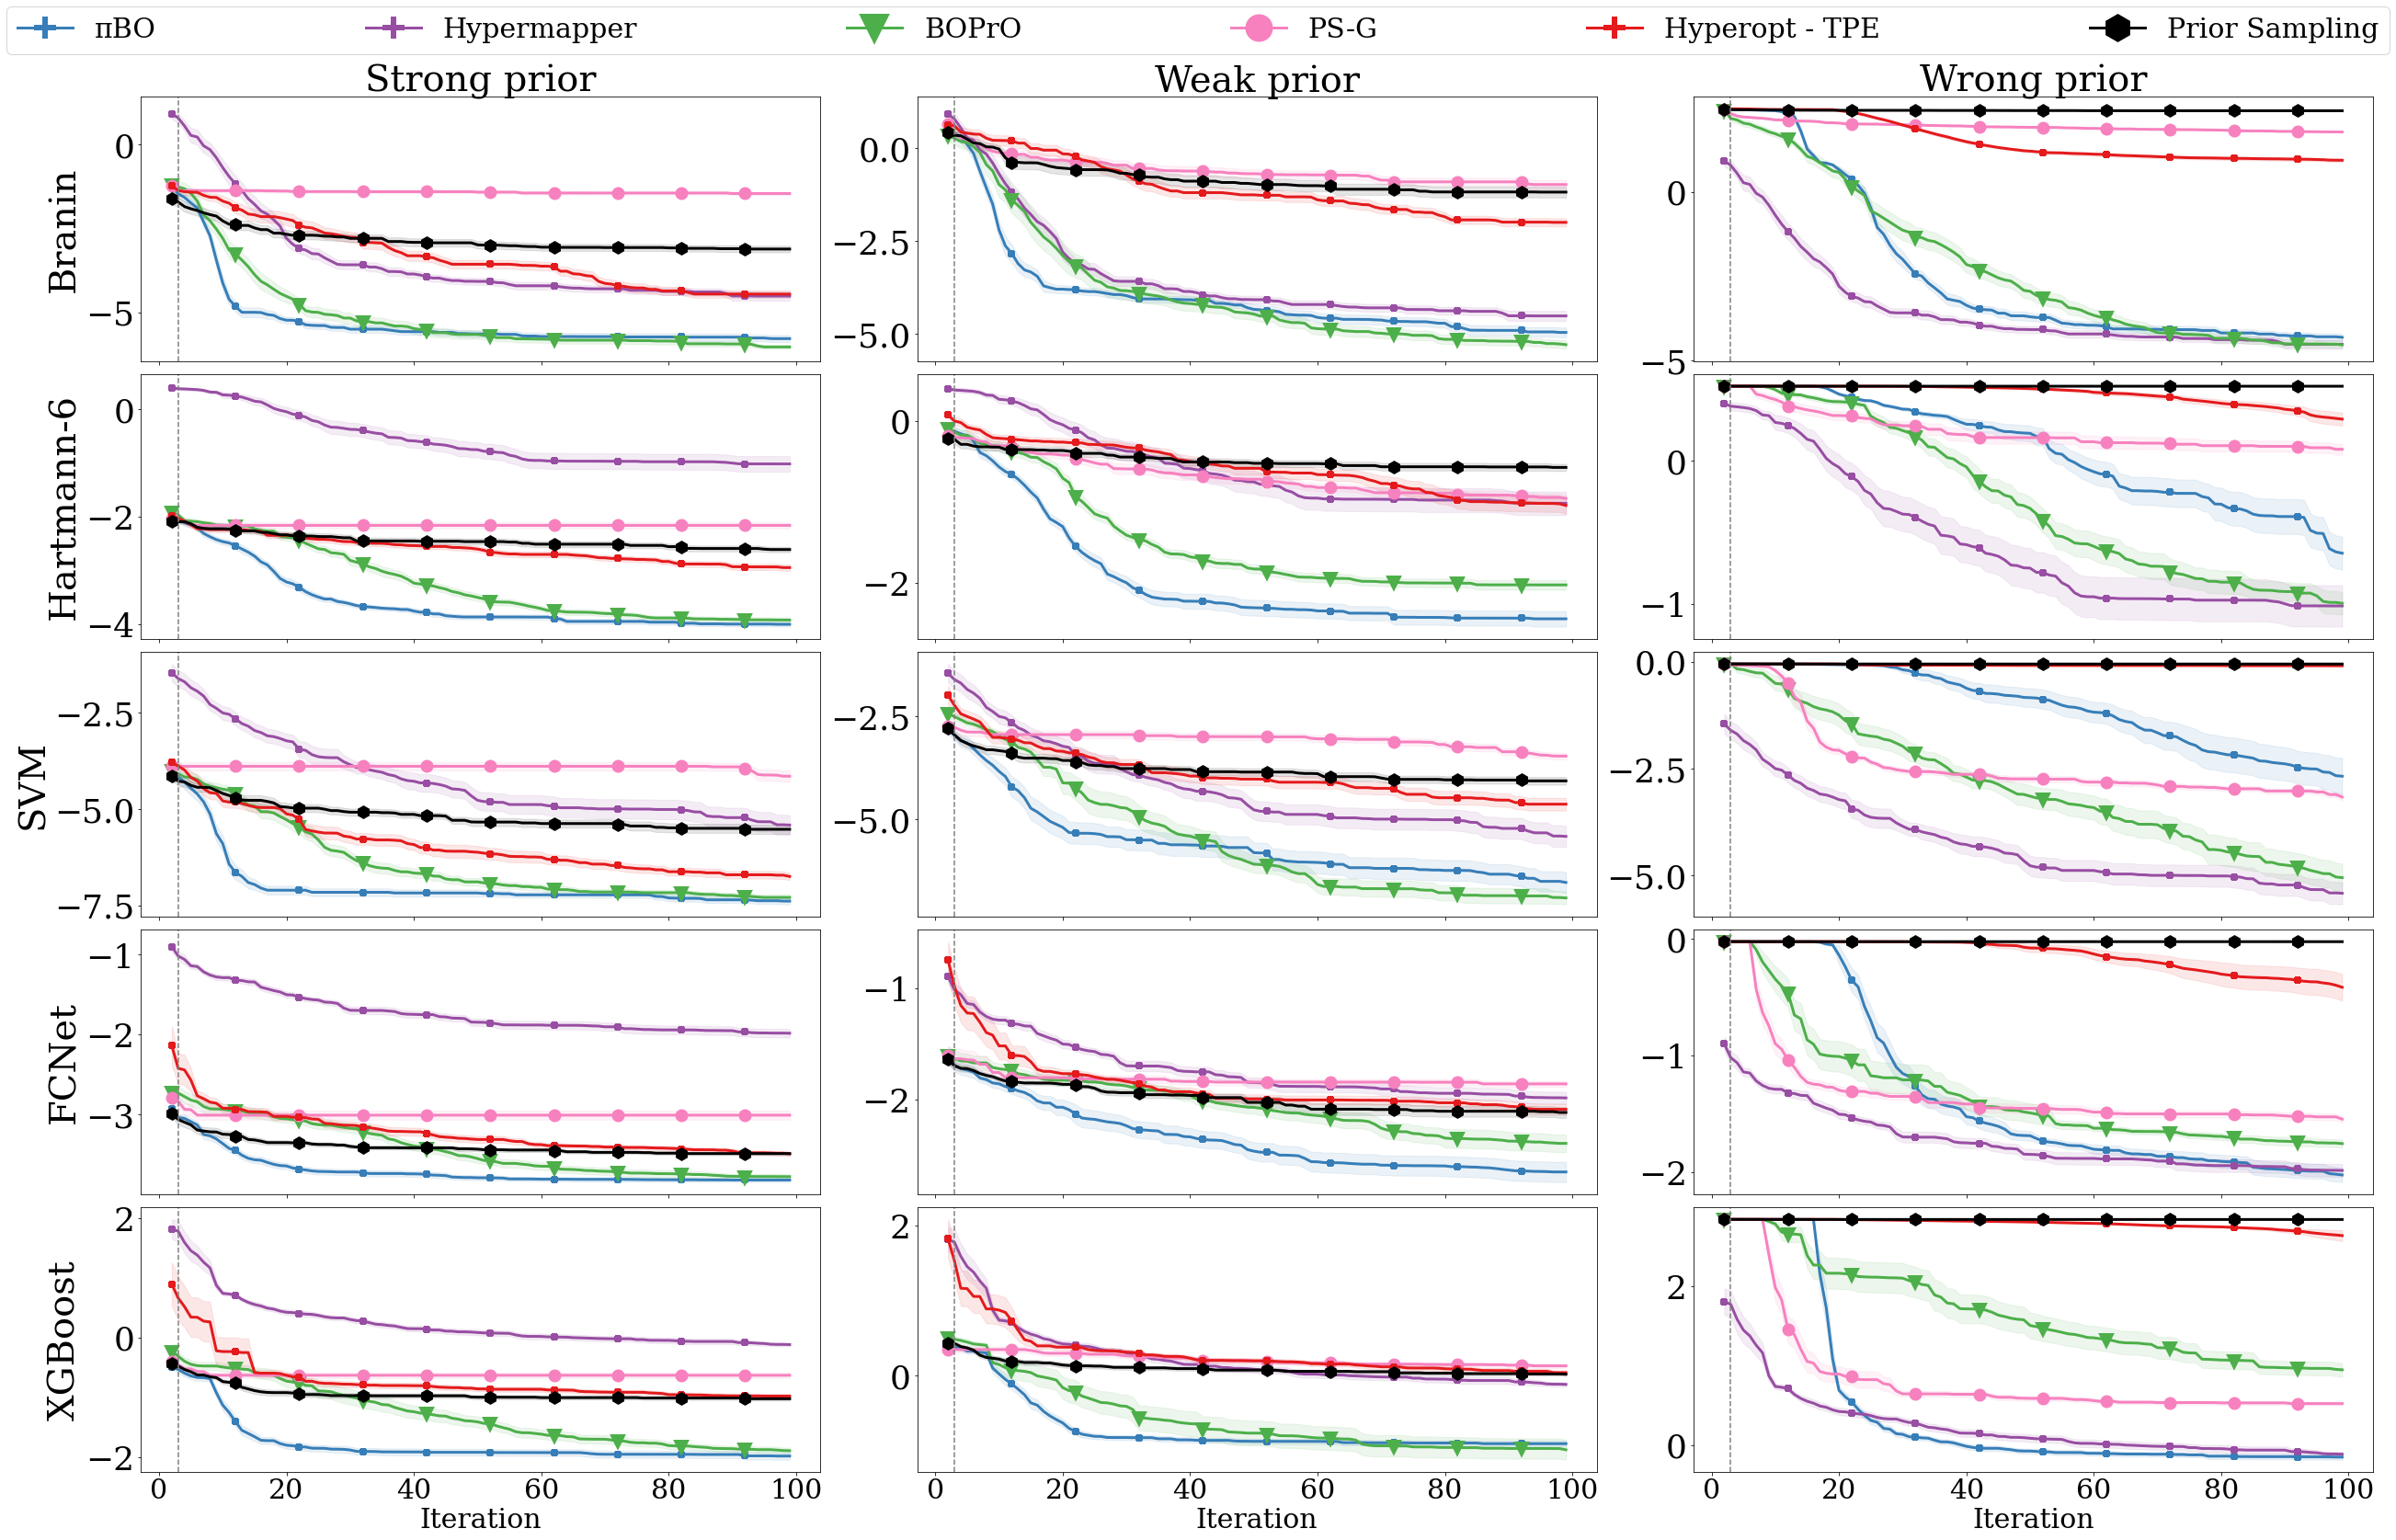
\includegraphics[width=\linewidth]{images/hypermapper_appendix.png}
    \caption{Comparison of \method{}, Hypermapper and other approaches for priors over the optimum for Branin, Hartmann and Profet benchmarks. \method{} is implemented in Spearmint. The mean and standard error of log simple regret is displayed over 100 iterations, averaged over 20 repetitions. Iteration 1 is removed for visibility purposes. The vertical line represents the end of the initial design phase.}
    \label{fig:appendix_hypermapper}
\end{figure}

\begin{figure}[tbph]
\centering
    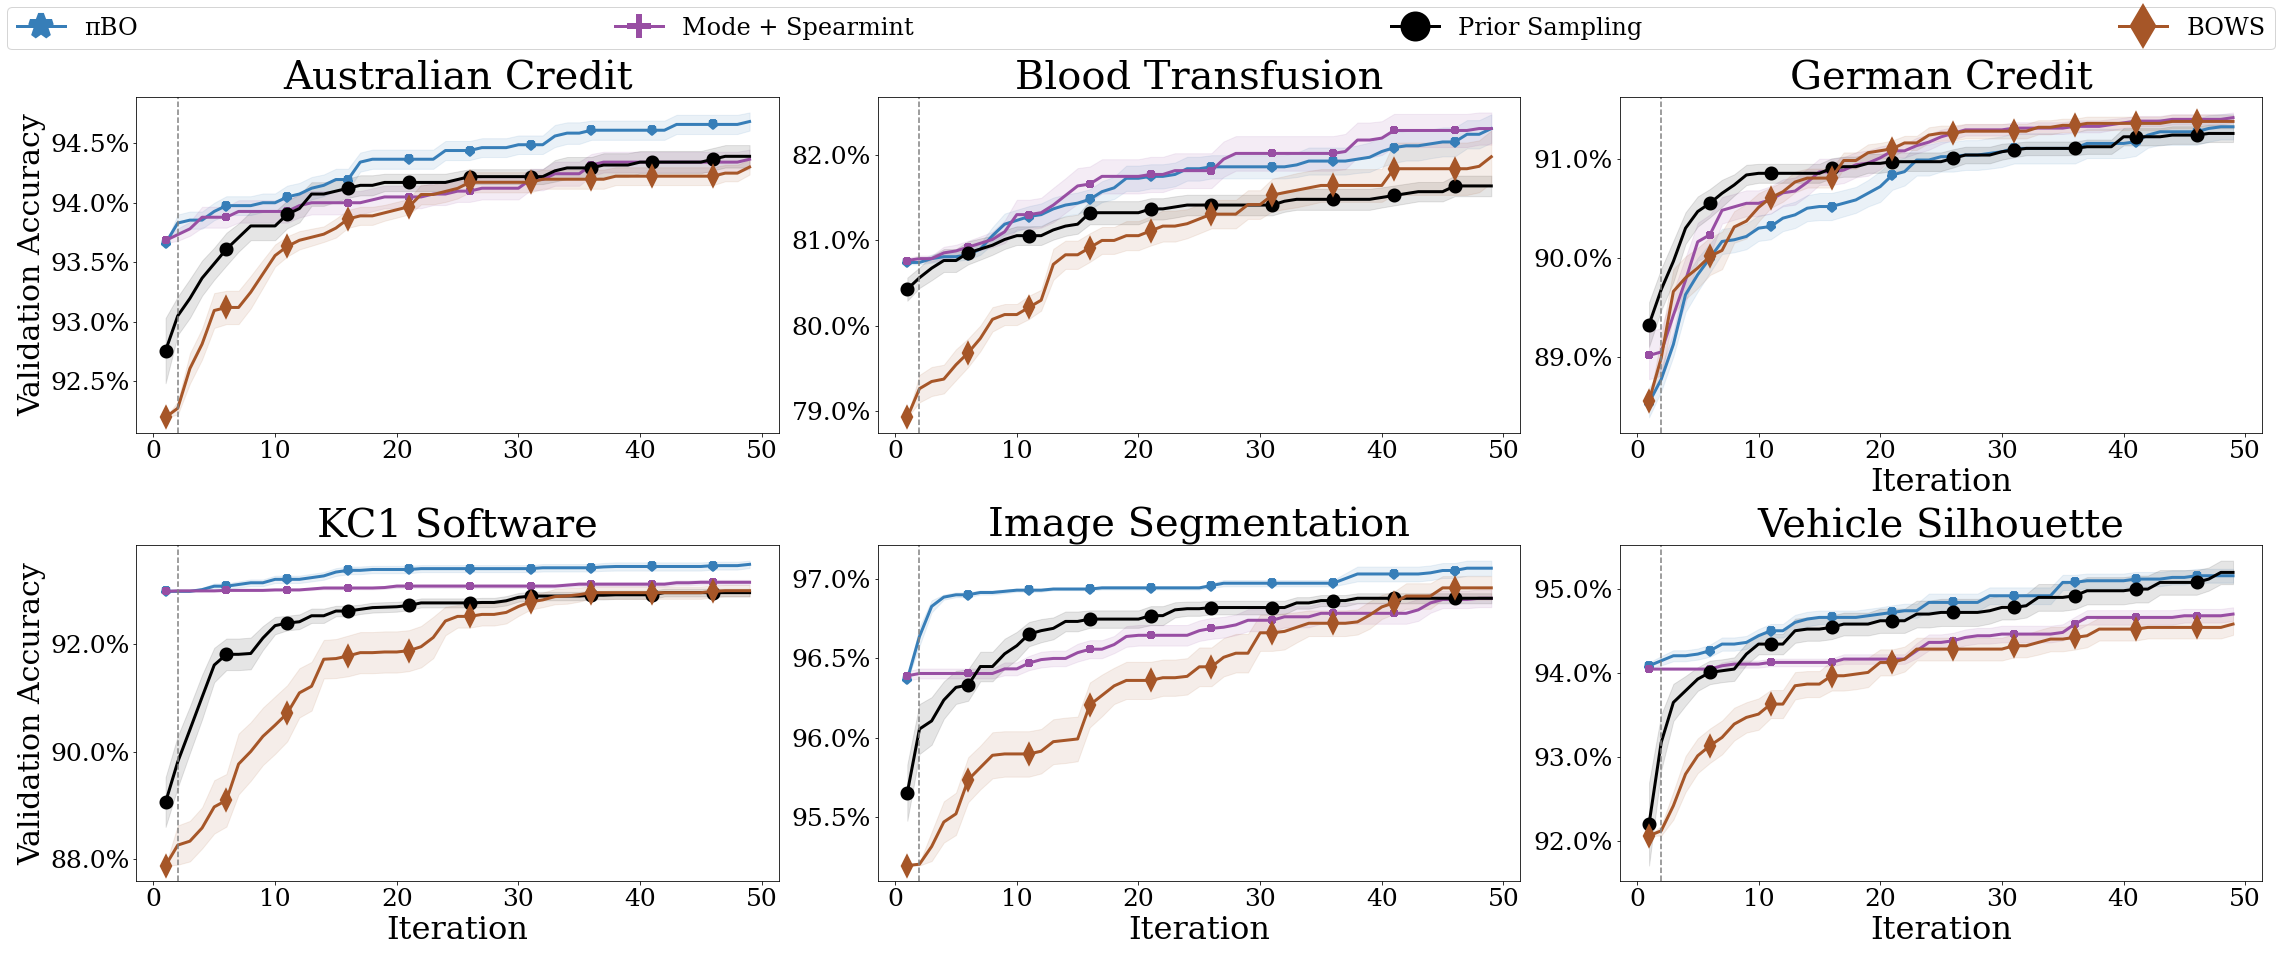
\includegraphics[width=\linewidth]{images/hpobench_sm.png}
    \caption{Comparison of \method{}, BOPrO, BOWS, and prior sampling for 5D MLP tuning on various OpenML datasets for a prior centered around default values. We show mean and standard error of the accuracy across 20 repetitions. Iteration 1 is removed for visibility purposes. The vertical line represents the end of the initial design phase.}
    \label{fig:mlp_results_appendix}
\end{figure}

\section{Prior Construction} \label{sec:priors}
We now present the method by which we construct our priors. For the synthetic benchmarks, we mimic~\citep{souza2021bayesian} by offsetting a Gaussian distribution from the optima. For our case studies, we choose a Gaussian prior with zero correlation between dimensions. This was required in order to have a simple, streamlined approach that was compatible with all frameworks. We constructed the priors once before conducting the experiments, and kept them fixed throughout.

\textbf{Synthetic and Surrogate-based HPO Benchmarks}\quad
For these benchmarks, the approximate optima of all included functions could be obtained in advance, either analytically or empirically through extensive sampling. Thus, the correctness of the prior is ultimately known in advance. For a function of dimensionality $d$ with optimum at ${\bm{x^*}}$, the strong and weak prior qualities were constructed by using a quality-specific noise term $\bm{\epsilon} = \{\epsilon_i\}_{i=1}^d$ and quality-specific standard deviation as a fraction of the search space. For the strong prior $\pri_s(\bm{x})$, we use a small standard deviation $\sigma_s = 1\%$ and construct the prior as

\begin{equation}
    \pri_s(\bm{x}) \sim \mathcal{N}(\bm{x^*+\epsilon}, \sigma_s), \quad \epsilon_i \sim\mathcal{N}(0, \sigma_s).
\end{equation}
We construct the weak priors analogously by using a larger standard deviation $\sigma_w = 10\%$. For our 20 runs of the strong and weak prior, this procedure yielded us 20 unique priors per quality type, with varying offsets from the true optimum. Additionally, the density on the optimum is substantially larger for the strong prior than the weak prior. No priors with a mean outside the search space were allowed, such priors were simply replaced. For Branin, we only considered one of the three Branin optima for this procedure, since not all included frameworks support multi-modal distributions. For the wrong prior, we construct it similarly to the strong prior, but around the empirical maximum, $\bm{x}^{\bar{*}}$, of the objective function in the search space. Since this point was far away from the optimum for all benchmarks, we did not add additional noise. So, the wrong prior $\pri_m$ is constructed as
\begin{equation}
    \pri_m(\bm{x}) \sim \mathcal{N}(\bm{x}^{\bar{*}}, \sigma_s),
\end{equation}
which means that the wrong prior is identical across runs for a given benchmark.

\section{Proofs} \label{sec:appendix_proof}
Here, we provide the complete proofs for the Theorem and Corollary introduced in \ref{sec:theory}. In addition, we provide insight into the interplay between $\beta$, the prior $\pi$, and the value of the derived bound  $C_{\pi, n}$.

%\subsection{Proof of Theorem 1}
\begin{customthm}{1}\label{one}
Given $\mathcal{D}_n$, $K_{\bm{\ell}}$, $\pri$, $\sigma$, ${\bm{\ell}}$, $R$ and the compact set $\mathcal{X}\subset\mathbb{R}^d$ as defined above, the loss $\mathcal{L}_{n}$ incurred at iteration $n$ by $\text{EI}_{\pri, n}$
can be bounded from above as
%Given $\mathcal{D}_n$, $K_{\bm{\ell}}$, $\pri$, $\sigma$, ${\bm{\ell}}$ and R, the loss $\mathcal{L}_{n}$ incurred at iteration $n$ by $\text{EI}_{\pri, n}$
%%when considering the next design point $\bm{x}_{n+1}$ 
% Given (everything mentioned above) this, this and this that as defined above,  - BR is ball, n is iteration in BO
%can be bounded from above as:
%by the loss incurred by vanilla EI, multiplied by a factor that tends to 1 as $n\rightarrow \infty$:
\begin{equation}
    \mathcal{L}_{n}(\text{EI}_{\pri, n}, \mathcal{D}_n, \mathcal{H}_{\bm{\ell}}(\mathcal{X}), R) \leq C_{\pi, n} \mathcal{L}_{n}(\text{EI}_n, \mathcal{D}_n, \mathcal{H}_{\bm{\ell}}(\mathcal{X}), R), \quad C_{\pi, n} = \left(\frac{\max_{\xinx} \pi(\bm{x})}{\min_{\xinx} \pi(\bm{x})}\right)^{\beta/n}.
\end{equation}
\end{customthm}

\begin{proof}
To bound the performance of \pei{} to that of EI, we primarily need to consider Lemma~7 and Lemma~8 by Bull \cite{JMLR:v12:bull11a}. In Lemma~7, it is stated that for any sequence of points $\{\bm{x}_i\}_{i=1}^n$, dimensionality $d$, kernel length scales ${\bm{\ell}}$, and $p \in \mathbb{N}$, the posterior variance $s^2_n$ 
on $\bm{x}_{n+1}$ will, for a large value $C$, satisfy the following inequality at most $p$ times, 
%can be bounded in the number of times $p$ that the variance exceeds a large value as
\begin{equation} \label{varbound}
    s_n(\bm{x}_{n+1}; \bm{\ell}) \geq Cp^{-(\nu \land 1)/d}(\log p)^\gamma, \quad \gamma = \begin{cases}
		\alpha, & \nu \leq 1\\
        0, & \nu > 1
	\end{cases}.
\end{equation}
%In other words, Lemma~7 says that \eqref{varbound} can only happen for $p$ of the $n$ total $x_i$. 
Thus, we can bound the posterior variance by assuming a point in time $n_p$ where Eq. \ref{varbound} has held $p$ times. 
We now consider Lemma 8 where, through a number of inequalities, EI is bounded by the actual improvement $I_n$
\begin{equation}
    \max\left(I_n-Rs, \frac{\tau(-R/\sigma)}{\tau(R/\sigma)}I_n   \right) \leq \eixn \leq I_n + (R + \sigma)s,
\end{equation}
where $I_n = (f(\bm{x}^*_n) - f(\bm{x}))^+$, $\tau(z) = z\Phi(z) + \phi(z)$ and $s = s_n(\bm{x}_{n}; \bm{\ell})$. Since \method re-weights $\text{EI}_n$ by $\pri_n$, these bounds need adjustment to hold for $\text{EI}_{\pi, n}$. 
For the upper bound provided in Lemma~8, we make use of $\max_{\xinx} \pri_n(\bm{x})$ to bound $\peixn$ %to $\eixn$ 
for any point $\xinx$: 
\begin{equation}
    \frac{\peixn} {\max_{\xinx} \pri_n(\bm{x})} = \frac{\eixn \pri_n(\bm{x})} {\max_{\xinx}\pri_n(\bm{x})} \leq \eixn \leq I_n + (R + \sigma)s.
\end{equation}
For the lower bounds, we instead rely on $\min_{\xinx} \pri_n(\bm{x})$ in a similar manner:
\begin{equation}
    \max\left(I_n-Rs, \frac{\tau(-R/\sigma)}{\tau(R/\sigma)}I_n   \right) \leq \eixn \leq \frac{\eixn \pri_n(\bm{x})} {\min_{\xinx}\pri_n(\bm{x})}  = \frac{\peixn} {\min_{\xinx} \pri_n(\bm{x})}.
\end{equation}
Consequently, \pei{} can be bounded by the actual improvement as
\begin{equation}
    {\min_{\xinx}\pri_n(\bm{x})}\max\left(I_n-Rs, \frac{\tau(-R/\sigma)}{\tau(R/\sigma)}I_n\right) \leq \peixn \leq {\max_{\xinx}\pri_n(\bm{x})} (I_n + (R + \sigma)s). 
\end{equation}
With these bounds in place, we consider the setting as in the proof for Theorem 2 in Bull \cite{JMLR:v12:bull11a}, which proves an upper bound for the EI strategy in the fixed kernel parameters setting. 
At an iteration $n_p, p \leq n_p \leq 3p$, the posterior variance will be bounded by $Cp^{-(\nu \land 1)/d}(\log p)^\gamma$. Furthermore, since $I_n \geq 0$ and $||f||_{\mathcal{H}_\ell(\mathcal{X}))} \leq R$, we can bound the total improvement as
\begin{equation}
    \sum_i I_i \leq \sum_i f(\bm{x}^*_{i}) - f(\bm{x}^*_{i+1}) \leq f(\bm{x}^*_1) - \min f \leq 2||f||_\infty \leq 2R,
\end{equation}
leaving us a maximum of $p$ times that $I_n \geq 2Rp^{-1}$. Consequently, both the posterior variance $s^2_{n_p}$ and the improvement $I_{n_p}$ are bounded at $n_p$. For a future iteration $n,\; 3p \leq n \leq 3(p+1)$, we use the  bounds on \pei, $s_{n_p}$ and $I_{n_p}$ to obtain the bounds on the \pei{} loss:
\begin{equation*} 
%\label{eq:bound_loss}
\begin{split}
    &\mathcal{L}_{n}(\text{EI}_\pri, \mathcal{D}_n, \mathcal{H}_{\bm{\ell}}(\mathcal{X}), R) \\
    &= f(\bm{x}_n^*) - \min f \\
    &\leq  f(\bm{x}_{n_p}^*) - \min f \\
    &\leq\frac{\text{EI}_{\pi,n_p}(\bm{x}^*)}{\min_{\xinx}\pri_n(\bm{x})}  \frac{\tau (R/\sigma)}{\tau (-R/\sigma)} \\
    &\leq
    \frac{\text{EI}_{\pi,n_p}(\bm{x}_{n+1})}{\min_{\xinx}\pri_n(\bm{x})}  \frac{\tau (R/\sigma)}{\tau (-R/\sigma)} \\
    &\leq\frac{\max_{\xinx}\pri_n(\bm{x})}{\min_{\xinx}\pri_n(\bm{x})}  \frac{\tau (R/\sigma)}{\tau (-R/\sigma)}
    \left(I_{n_p} + (R+\sigma)s_{n_p}\right)\\
    &\leq\left(\frac{\max_{\xinx}\pri(\bm{x})}{\min_{\xinx}\pri(\bm{x})}\right)^{\beta/n}  \frac{\tau (R/\sigma)}{\tau (-R/\sigma)} (2Rp^{-1} + (R+\sigma)Cp^{-(\nu \land 1)/d}(\log p)^\gamma),
\end{split}
\end{equation*}
where the last inequality 
%in Eq. \ref{eq:bound_loss} 
is a factor $C_{\pri, n} = \left(\frac{\max_{\xinx}\pri(\bm{x})}{\min_{\xinx}\pri(\bm{x})}\right)^{\beta/n}$ larger than the bound on $\mathcal{L}_n(\text{EI}, \mathcal{D}_n, \mathcal{H}_{\bm{\ell}}(\mathcal{X}), R)$.
\end{proof} 


%\subsection{Proof of Corollary 1}
\begin{customcorl}{1}\label{corollaryone}
The loss of a decaying prior-weighted Expected Improvement strategy, \pei{}, is asymptotically equal to the loss of an Expected Improvement strategy, EI:
\begin{equation}
    \mathcal{L}_{n}(\text{EI}_{\pri, n}, \mathcal{D}_n, \mathcal{H}_{\bm{\ell}}(\mathcal{X}), R) \sim  \mathcal{L}_{n}(\text{EI}_n, \mathcal{D}_n, \mathcal{H}_{\bm{\ell}}(\mathcal{X}), R),
\end{equation}

so we obtain a convergence rate for \pei{} of $\mathcal{L}_{n}(\text{EI}_{\pri, n}, \mathcal{D}_n, \mathcal{H}_{\bm{\ell}}(\mathcal{X}), R) = \mathcal{O}(n^{-(\nu \land 1)/d}(\log n)^\gamma)$.
\end{customcorl}

\begin{proof}
We simply compute the fraction of the losses in the limit,
\begin{equation}
    \lim_{n \to \infty}\frac{\mathcal{L}_n(\text{EI}_\pi, \mathcal{D}_n, \mathcal{H}_{\bm{\ell}}(\mathcal{X}), R)}{\mathcal{L}_n(\text{EI}, \mathcal{D}_n, \mathcal{H}_{\bm{\ell}}(\mathcal{X}), R)} \le \lim_{n \to \infty} \left(\frac{\max_{\xinx}\pri(\bm{x})}{\min_{\xinx}\pri(\bm{x})}\right)^{\beta/n} =1.
\end{equation}
\end{proof}

\subsection{Sensitivity analysis on $C_{\pri, n}$}
We now provide additional insight into how $C_{\pri, n}$ depends on the choices of prior and $\beta$ made by the user. To do so, we consider a typical low-budget setting and display values of $C_{\pri, n}$ at iteration 50. We consider a one-dimensional search space where with a Gaussian prior located in the center of the search space. In the plot below, we display how the choice of $\sigma$, given as a percentage of the search space, and $\beta$, the prior confidence parameter, yield different values of $C_{\pri, n}$. We see that, for approximately half of the space, the upper bound on the loss is at least 80\% (bright green or yellow) of the upper bound of EI, and only a small region of very narrow priors (dark blue) give a low guaranteed convergence rate.

\begin{figure}[h]
    \centering
    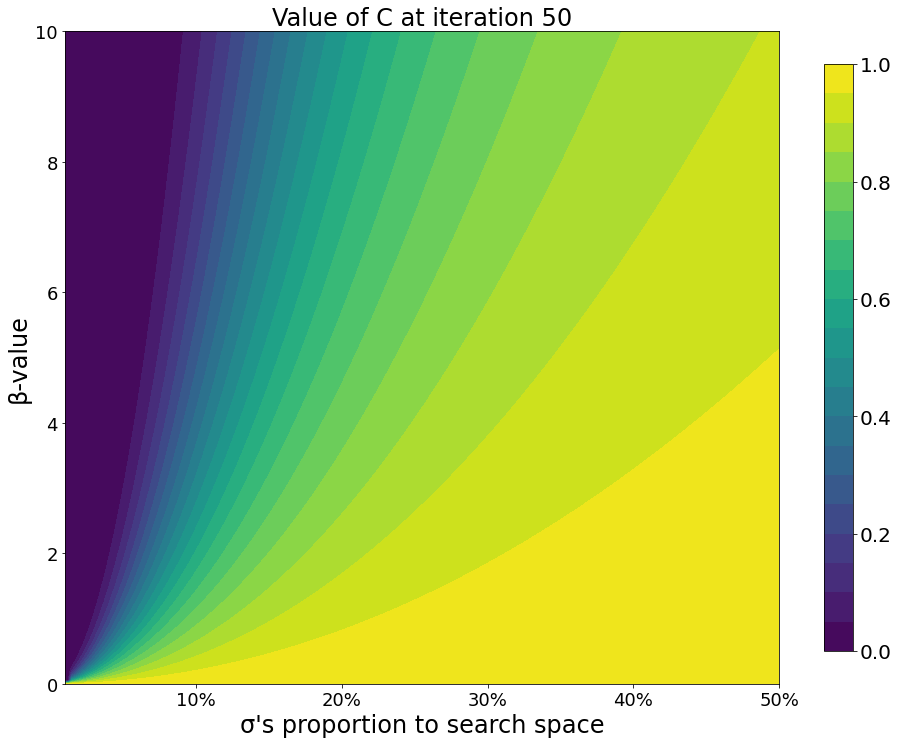
\includegraphics[width=0.7\linewidth]{images/c_value.png}
    \caption{Value of $C_{\pri, n}$ at iteration 50 for a centered Gaussian prior in a one-dimensional search space, varying $\sigma$ and $\beta$. The value of $C_{\pri, n}$ upper bounds the loss incurred by \pei relative EI at the at the given iteration, given the same data. Regions in dark represent pairs of ($\sigma, \beta$) where the upper bound on prior-weighted EI is low relative to EI, whereas regions in yellow represent pairs of ($\sigma, \beta$) where the upper bound is approximately the same.}
    \label{fig:appendix_hypermapper}
\end{figure}

\section{Experiment Details} \label{sec:experiments_appendix}
%In this section, we provide descriptions of the benchmarks and case studies used, as well as their associated priors and resources used.
\subsection{Frameworks} \label{sec:implementation}
Our implementations of \method require little change in the supporting frameworks, Spearmint and HyperMapper, and we stay as close to the default settings as possible for each framework. For both Spearmint and HyperMapper, we consider a Matérn 5/2 Kernel. For particularly strong priors, rounding errors can cause the prior to be zero in parts of the search space, potentially affecting \method's convergence properties. To avoid these rounding errors and ensure a strictly positive prior, we add a small constant, $\epsilon=10^{-12}$, to the prior throughout the search space for all prior qualities. 
For the initial sampling from the prior, we truncate the distribution by disallowing sampled points from outside the search space, instead re-sampling such points. During optimization, we do not to explicitly truncate the prior, as points outside the search space are never considered during acquisition function maximization. Thus, the prior is effectively truncated to fit the search space without requiring additional consideration.


 To the best of our knowledge, there is no publicly available implementation of BOWS, so we re-implemented it in Spearmint. For the Spearmint implementation of BOWS,
%, we similarly rely on the default settings to as great an extent as possible. W
we provide warped versions of each benchmark, obtaining 20 unique warpings per prior quality and benchmark. We truncate the prior by restricting the warped search space to only include the region which maps back to the original search space through the inverted warping function. For all other approaches, we use the original, publicly available implementations. Notably, the available implementation of Hyperopt TPE does not support bounded search spaces under our priors; as a compromise, when asked to evaluate outside the search space we return an empirically obtained maximum on the objective function inside the search space.
 
 We use the search spaces, prior locations and descriptions used by ~\citep{souza2021bayesian} for the toy and surrogate HPO problems.
%\danny{Wasnt this appendix E at some point? As we can not change the main paper file, we should make sure to not mix up }
%\carl{In the last turn-in, this was actually the orfder}
We now provide additional details about the benchmarks and case study tasks used, their associated search spaces and priors, and the resources used to run these studies.

\subsection{Benchmarks and Case Studies}

\textbf{Branin}\quad The Branin function is a well-known synthetic benchmark for optimization problems. The Branin function has two input dimensions and three global minima. %The Branin function is defined as:

\textbf{Hartmann-6}\quad The Hartmann-6 function is a well-known synthetic benchmark for optimization problems, which has one global optimum and six dimensions. %The Branin function is defined as:

\textbf{SVM}\quad A hyperparameter-optimization benchmark in 2D based on Profet~\citep{profet}. This benchmark is generated by a generative meta-model built using a set of SVM classification models trained on 16 OpenML tasks. The benchmark has two input parameters, corresponding to SVM hyperparameters.

\textbf{FCNet}\quad A hyperparameter and architecture optimization benchmark in 6D based on Profet. The FC-Net benchmark is generated by a generative meta-model built using a set of feed-forward neural networks trained on the same 16 OpenML tasks as the SVM benchmark. The benchmark has six input parameters corresponding to network hyperparameters.

\textbf{XGBoost}\quad A hyperparameter-optimization benchmark in 8D based on Profet. The XGBoost benchmark is generated by a generative meta-model built using a set of XGBoost regression models in 11 UCI datasets. The benchmark has eight input parameters, corresponding to XGBoost hyperparameters.
%\carl{Am I allowed to copy this from BOPrO?}
%\danny{When one copies text there has to be a citation (even if its your own text)}

\textbf{OpenML MLP}\quad The OpenML MLP tuning tasks are provided through HPOBench\cite{eggensperger2021hpobench}, and train binary classifiers on real-world datasets. The 5D parameter space consists of four continous parameters and one integer parameter.

\textbf{U-Net Medical}\quad
The U-Net \citep{ronne2015unet} is a popular convolutional neural network architecture for image segmentation. We use the implementation and evaluation setting from the popular NVIDIA deep learning examples repository \citep{nvidiaexamples} to build a case study for optimizing hyperparameters for U-Net. The NVIDIA repository is aimed towards the segmentation of neuronal processes in electron microscopy images for the 2D EM segmentation challenge dataset \citep{unetdata1,unetdata2}. We optimize 6 hyperparameters of the U-Net pipeline.


\textbf{ImageNette}\quad
ImageNette \citep{imagenette} is a subset of 10 classes of ImageNet~\citep{deng2009imagenet} and is primarily used for algorithm development for the popular FastAI library~\citep{howard2018fastai}. The FastAI library contains a convolutional neural network pipeline for ImageNette, that is used by all competitors on the ImageNette leaderboard. We base our case study on the 80 epoch, 128 resolution setting of this leaderboard and optimize 6 of the hyperparameters of the FastAI ImageNette pipeline.


\subsection{Search Spaces and Priors}
The search spaces for each benchmark are summarized in Table~\ref{tab:benchmarks.space} (Branin and Profet), Table~\ref{tab:mlp.space} (OpenML MLP), and Table~\ref{tab:case_studies.space} (ImageNette and U-Net). For the Profet benchmarks, we report the original ranges and whether or not a log scale was used. However, in practice, Profet's generative model transforms the range of all hyperparameters to a linear $[0, 1]$ range. We use Emukit's public implementation for these benchmarks~\citep{emukit2019}.

\begin{table}[tb]
    \begin{center}
        \caption{Search spaces for the Branin and Profet benchmarks. We report the original ranges and whether or not a log scale was used. Mean of the strong and weak priors before offset are reported.
        }
        \label{tab:benchmarks.space}
        \begin{tabular}{lllll}
        \toprule
        \textbf{Benchmark} & \textbf{Range} & \textbf{Parameter values} & \textbf{Log scale} & \textbf{Prior mean}\\ \midrule
        Branin             & $x_1$                   & $[-5, 10]$                & -                  &$\pi$\\
                           & $x_2$                   & $[0, 15]$                 & -                  &$2.275$\\ \midrule
        SVM                & C                       & $[e^{-10}, e^{10}]$       & \checkmark         &$e^{7.84}$\\
                           & $\gamma$                & $[e^{-10}, e^{10}]$       & \checkmark         &$e^{-9.35}$\\ \midrule
        FCNet              & learning rate           & $[10^{-6}, 10^{-1}]$      & \checkmark         &$10^{-6}$\\
                           & batch size              & $[8, 128]$                & \checkmark         &$8.7$\\
                           & units layer 1           & $[16, 512]$               & \checkmark         &$210$\\
                           & units layer 2           & $[16, 512]$               & \checkmark         &$205$\\
                           & dropout rate l1         & $[0.0, 0.99]$             & -                  &$0.0007$\\
                           & dropout rate l2         & $[0.0, 0.99]$             & -                  &$0.852$\\ \midrule
        XGBoost            & learning rate           & $[10^{-6}, 10^{-1}]$      & \checkmark         &$10^{-6}$\\
                           & gamma                   & $[0,2]$                   & -                  &$2$\\
                           & L1 regularization       & $[10^{-5}, 10^{3}]$       & \checkmark         &$10^{0.088}$\\
                           & L2 regularization       & $[10^{-5}, 10^{3}]$       & \checkmark         &$10^{-1.78}$\\
                           & number of estimators    & $[10, 500]$               & -                  &$500$\\
                           & subsampling             & $[0.1, 1]$                & -                  &$0.1$\\
                           & maximum depth           & $[1, 15]$                 & -                  &$1$\\
                           & minimum child weight    & $[0, 20]$                 & -                  &$8.42$\\
                           \bottomrule
        \end{tabular}
    \end{center}
\end{table}

\begin{table}[tb]
    \begin{center}
        \caption{Search spaces for the two case studies. We report the original ranges and whether or not a log scale was used. Mean and standard deviation of the priors are reported, where the standard deviation is reported as a percentage of the search space. For the categorical variable pooling, the probabilities for activation functions in U-Net were set to uniform and the probabilities for pooling, $[$Avg, Max$]$,  were set to $[0.2, 0.8]$, respectively.}
        \label{tab:mlp.space}
        \begin{tabular}{llllll}
        \toprule
        \textbf{Benchmark} & \textbf{Parameter name} & \textbf{Range} & \textbf{Log scale} & \textbf{Prior mean} & \textbf{Prior st.dev.}\\\midrule
        OpenML MLP     & alpha           & $[10^{-6}, 10^{-2}]$       & \checkmark         & $10^{-4}$ & $25\%$\\ 
                           & batch size            & $[10^{-6}, 10^{-2}]$       & \checkmark         & $10^{-4.5}$ &$25\%$\\
                           & depth            & $\{1, 2, 3\}$       & -         & $0.5$ &$25\%$\\
                           & initial learning rate & $[0.6, 0.99]$       & \checkmark         & $0.9$ &$25\%$\\
                           & width            & $[0.9, 0.9999]$       & \checkmark         & $0.999$ &$25\%$\\
                           \bottomrule
        \end{tabular}
    \end{center}
\end{table}

\begin{table}[H]
    \begin{center}
        \caption{Search spaces for the two case studies. We report the original ranges and whether or not a log scale was used. Mean and standard deviation of the priors are reported, where the standard deviation is reported as a percentage of the search space. For the categorical variable pooling, the probabilities for activation functions in U-Net were set to uniform and the probabilities for pooling, $[$Avg, Max$]$,  were set to $[0.2, 0.8]$, respectively.}
        \label{tab:case_studies.space}
        \begin{tabular}{llllll}
        \toprule
        \textbf{Benchmark} & \textbf{Parameter name} & \textbf{Range} & \textbf{Log scale} & \textbf{Prior mean} & \textbf{Prior st.dev.}\\\midrule
        U-Net Medical      & learning rate           & $[10^{-6}, 10^{-2}]$       & \checkmark         & $10^{-4}$ & $25\%$\\ 
                           & weight decay            & $[10^{-6}, 10^{-2}]$       & \checkmark         & $10^{-4.5}$ &$25\%$\\
                           & dropout            & $[0, 0.99]$       & -         & $0.5$ &$25\%$\\
                           & $\beta_1$           & $[0.6, 0.99]$       & \checkmark         & $0.9$ &$25\%$\\
                           & $\beta_2$            & $[0.9, 0.9999]$       & \checkmark         & $0.999$ &$25\%$\\
                           & activation            & 3 options\footnote{$\{$ReLU, Leaky ReLU, SELU$\}$}       & -        & - &$25\%$\\
                           \midrule
        ImageNette-128     & learning rate           & $[10^{-4}, 0]$             & \checkmark         & $10^{-2.10}$ & $25\%$\\
                           & squared momentum        & $[0.9, 0.999]$             & \checkmark         & $0.99$ &$25\%$\\
                           & momentum                & $[0, 0.99]$               & -                  & $0.95$ &$25\%$\\
                           & epsilon                 & $[10^{-7}, 10^{-5}]$       & \checkmark         & $10^{-6}$ &$25\%$\\
                           & mixup                   & $[0.0, 0.5]$              & -                  & $0.4$ &$25\%$\\
                           & pooling                 & $\{$Avg, Max$\}$              & -                  & - & - \\ \bottomrule
        \end{tabular}
    \end{center}
\end{table}

\subsection{Case Study Details}

% Did you specify all the training details (e.g., data splits, hyperparameters, how they were chosen)?
\paragraph{Training details deep learning case studies} Both case studies are based on existing deep learning code, whose hyperparameters we vary according to the HPO. In both case studies, we enabled mixed precision training, and for ImageNette-128 to work in conjunction with Spearmint, we had to enable the MKL\_SERVICE\_FORCE\_INTEL environment flag. For all further details, we refer to the supplementary material containing our code.

% Did you include the total amount of compute and the type of resources used (e.g., type of GPUs, internal cluster, or cloud provider)?

\paragraph{Resources used for deep learning case studies}
For U-Net Medical we used one GeForce RTX 2080 Ti GPU, whereas for ImageNette-128 we used two GeForce RTX 2080 Ti GPU's. Also, we used 4 cores and 8 cores respectively, of an AMD EPYC 7502 32-Core Processor. In Table \ref{tab:computeused} we list the GPU hours needed for running the deep learning case studies as well as the emitted CO$_2$ equivalents.

\begin{table}[H]
    \begin{center}
        \caption{Approximate GPU hours required to perform an evaluation for one approach for the deep learning case studies. Additionally we report approximate carbon footprints using the \href{https://mlco2.github.io/impact\#compute}{MachineLearning Impact calculator} presented in \cite{lacoste2019quantifying} based on OECD's 2014 yearly average carbon efficiency.}
        \label{tab:computeused}
        \begin{tabular}{lllll}
        \toprule
        \textbf{Benchmark} & \textbf{Repetitions} & \textbf{GPUh's Per Repetition} & \textbf{Total GPUh} & \textbf{Total kgCO$_2$eq} \\\midrule
        U-Net Medical      & 20 & 9 & 180 & 19.4 \\
        ImageNette-128     & 10 & 40 & 400 & 43.2 \\ \bottomrule
        \end{tabular}
    \end{center}
\end{table}


\paragraph{Assets deep learning case studies}
% If your work uses existing assets, did you cite the creators? code, data, and models
In addition to the assets we list in the main paper, the U-Net Medical code base we used employs the 2D EM segmentation challenge dataset \citep{unetdata1,unetdata2}, which is available for for the purpose of generating or testing non-commercial image segmentation software. We include licenses of all existing code assets we used in the supplementary material containing our code.

\section{Sensitivity to Prior Strength} \label{sec:ablation_prior}

We investigate the performance of \method{} when providing priors over the optimum of various qualities. To show the effect of decreasing the prior strength, a grid of prior qualities, with varying widths and offsets from the optimum, are provided. Thus, priors range from the strong prior in the results, to weak, correct priors and sharp, misplaced priors.

From Figures~\ref{fig:branin_grid}-~\ref{fig:xgboost_grid}, it is shown that \method{} provides substantial performance across most prior qualities for all benchmarks but Branin, and recoups its early losses on the worst priors in the bottom left corner. \method{} demonstrates sensitivity to the width of the prior, as the optimization does not progress as quickly for well-located priors with a larger width. Additionally, \method{}'s improvement over the Spearmint + Mode baseline is further emphasized, as this baseline often fails to meaningfully improve over the mode in early iterations.  

\begin{figure}
    \centering
    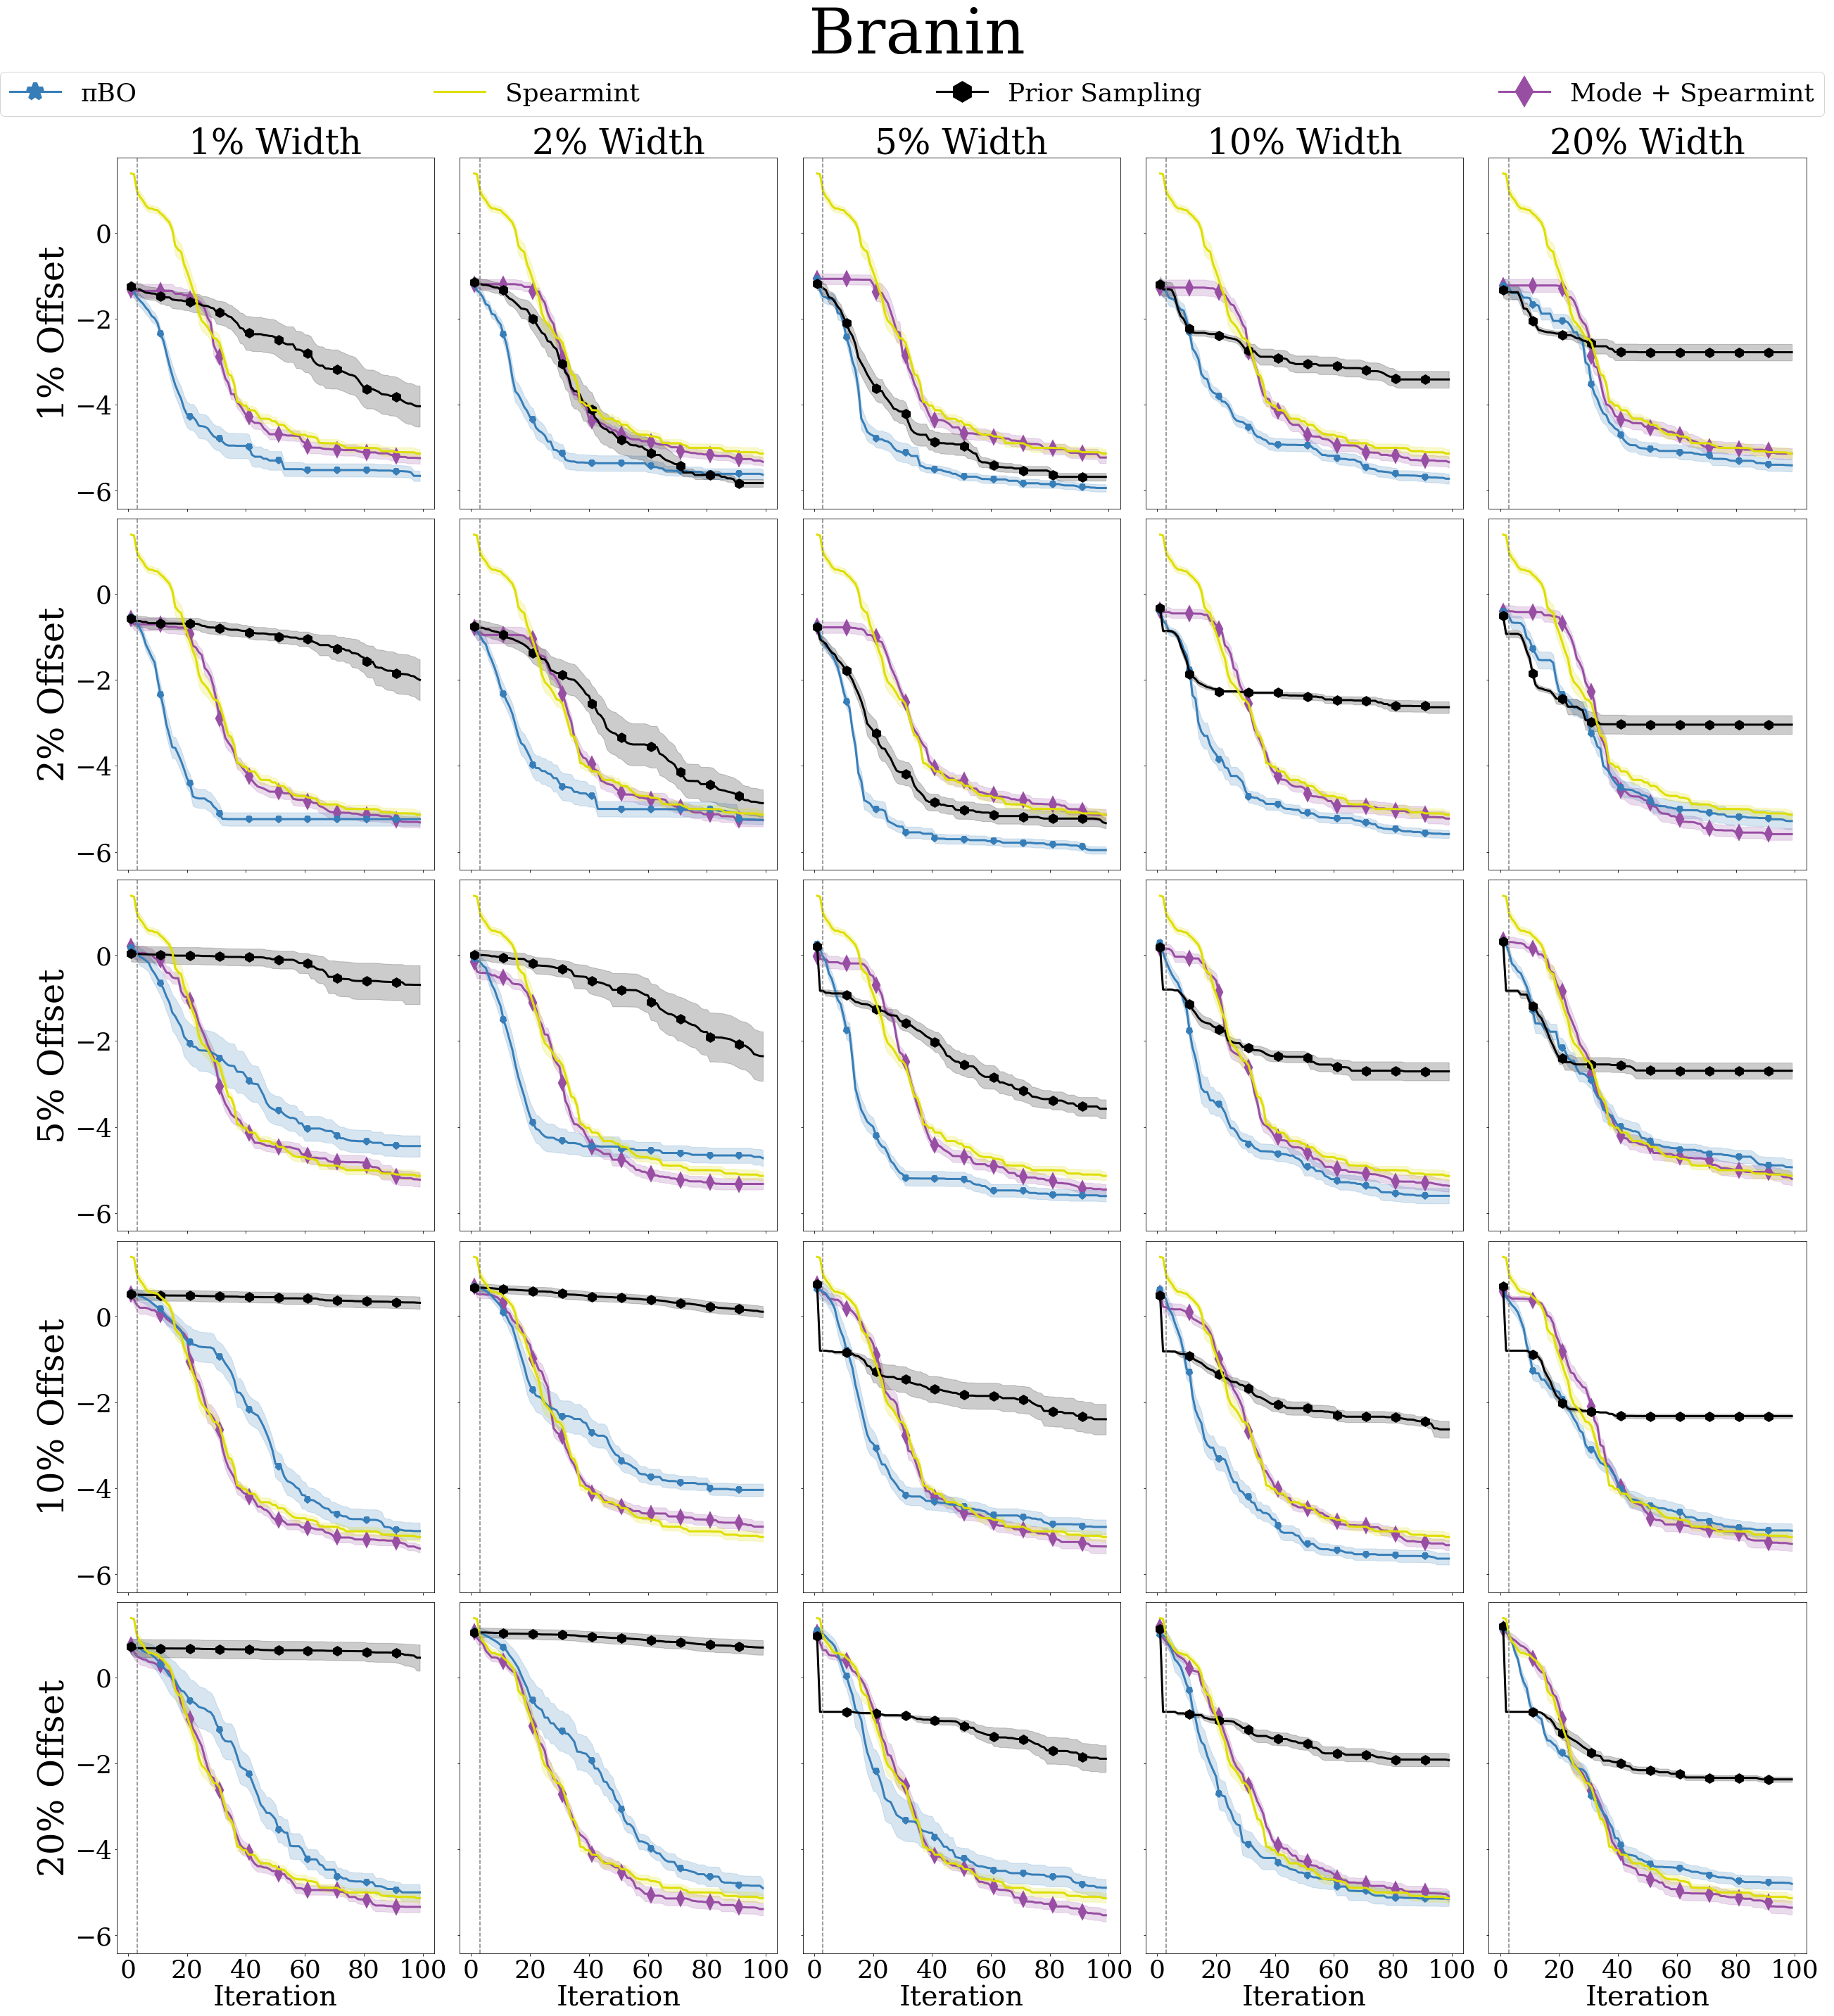
\includegraphics[width=\linewidth]{images/branin_grid.png}
    \caption{Comparison on Branin of priors with varying widths and offsets over the optimum on \method{}, Spearmint, Spearmint with mode initialization, and sampling from the prior. The mean and standard error of log simple regret is displayed over 100 iterations, averaged over 20 repetitions. Iteration 1 is removed for visibility purposes.}
    \label{fig:branin_grid}
\end{figure}

\begin{figure}
    \centering
    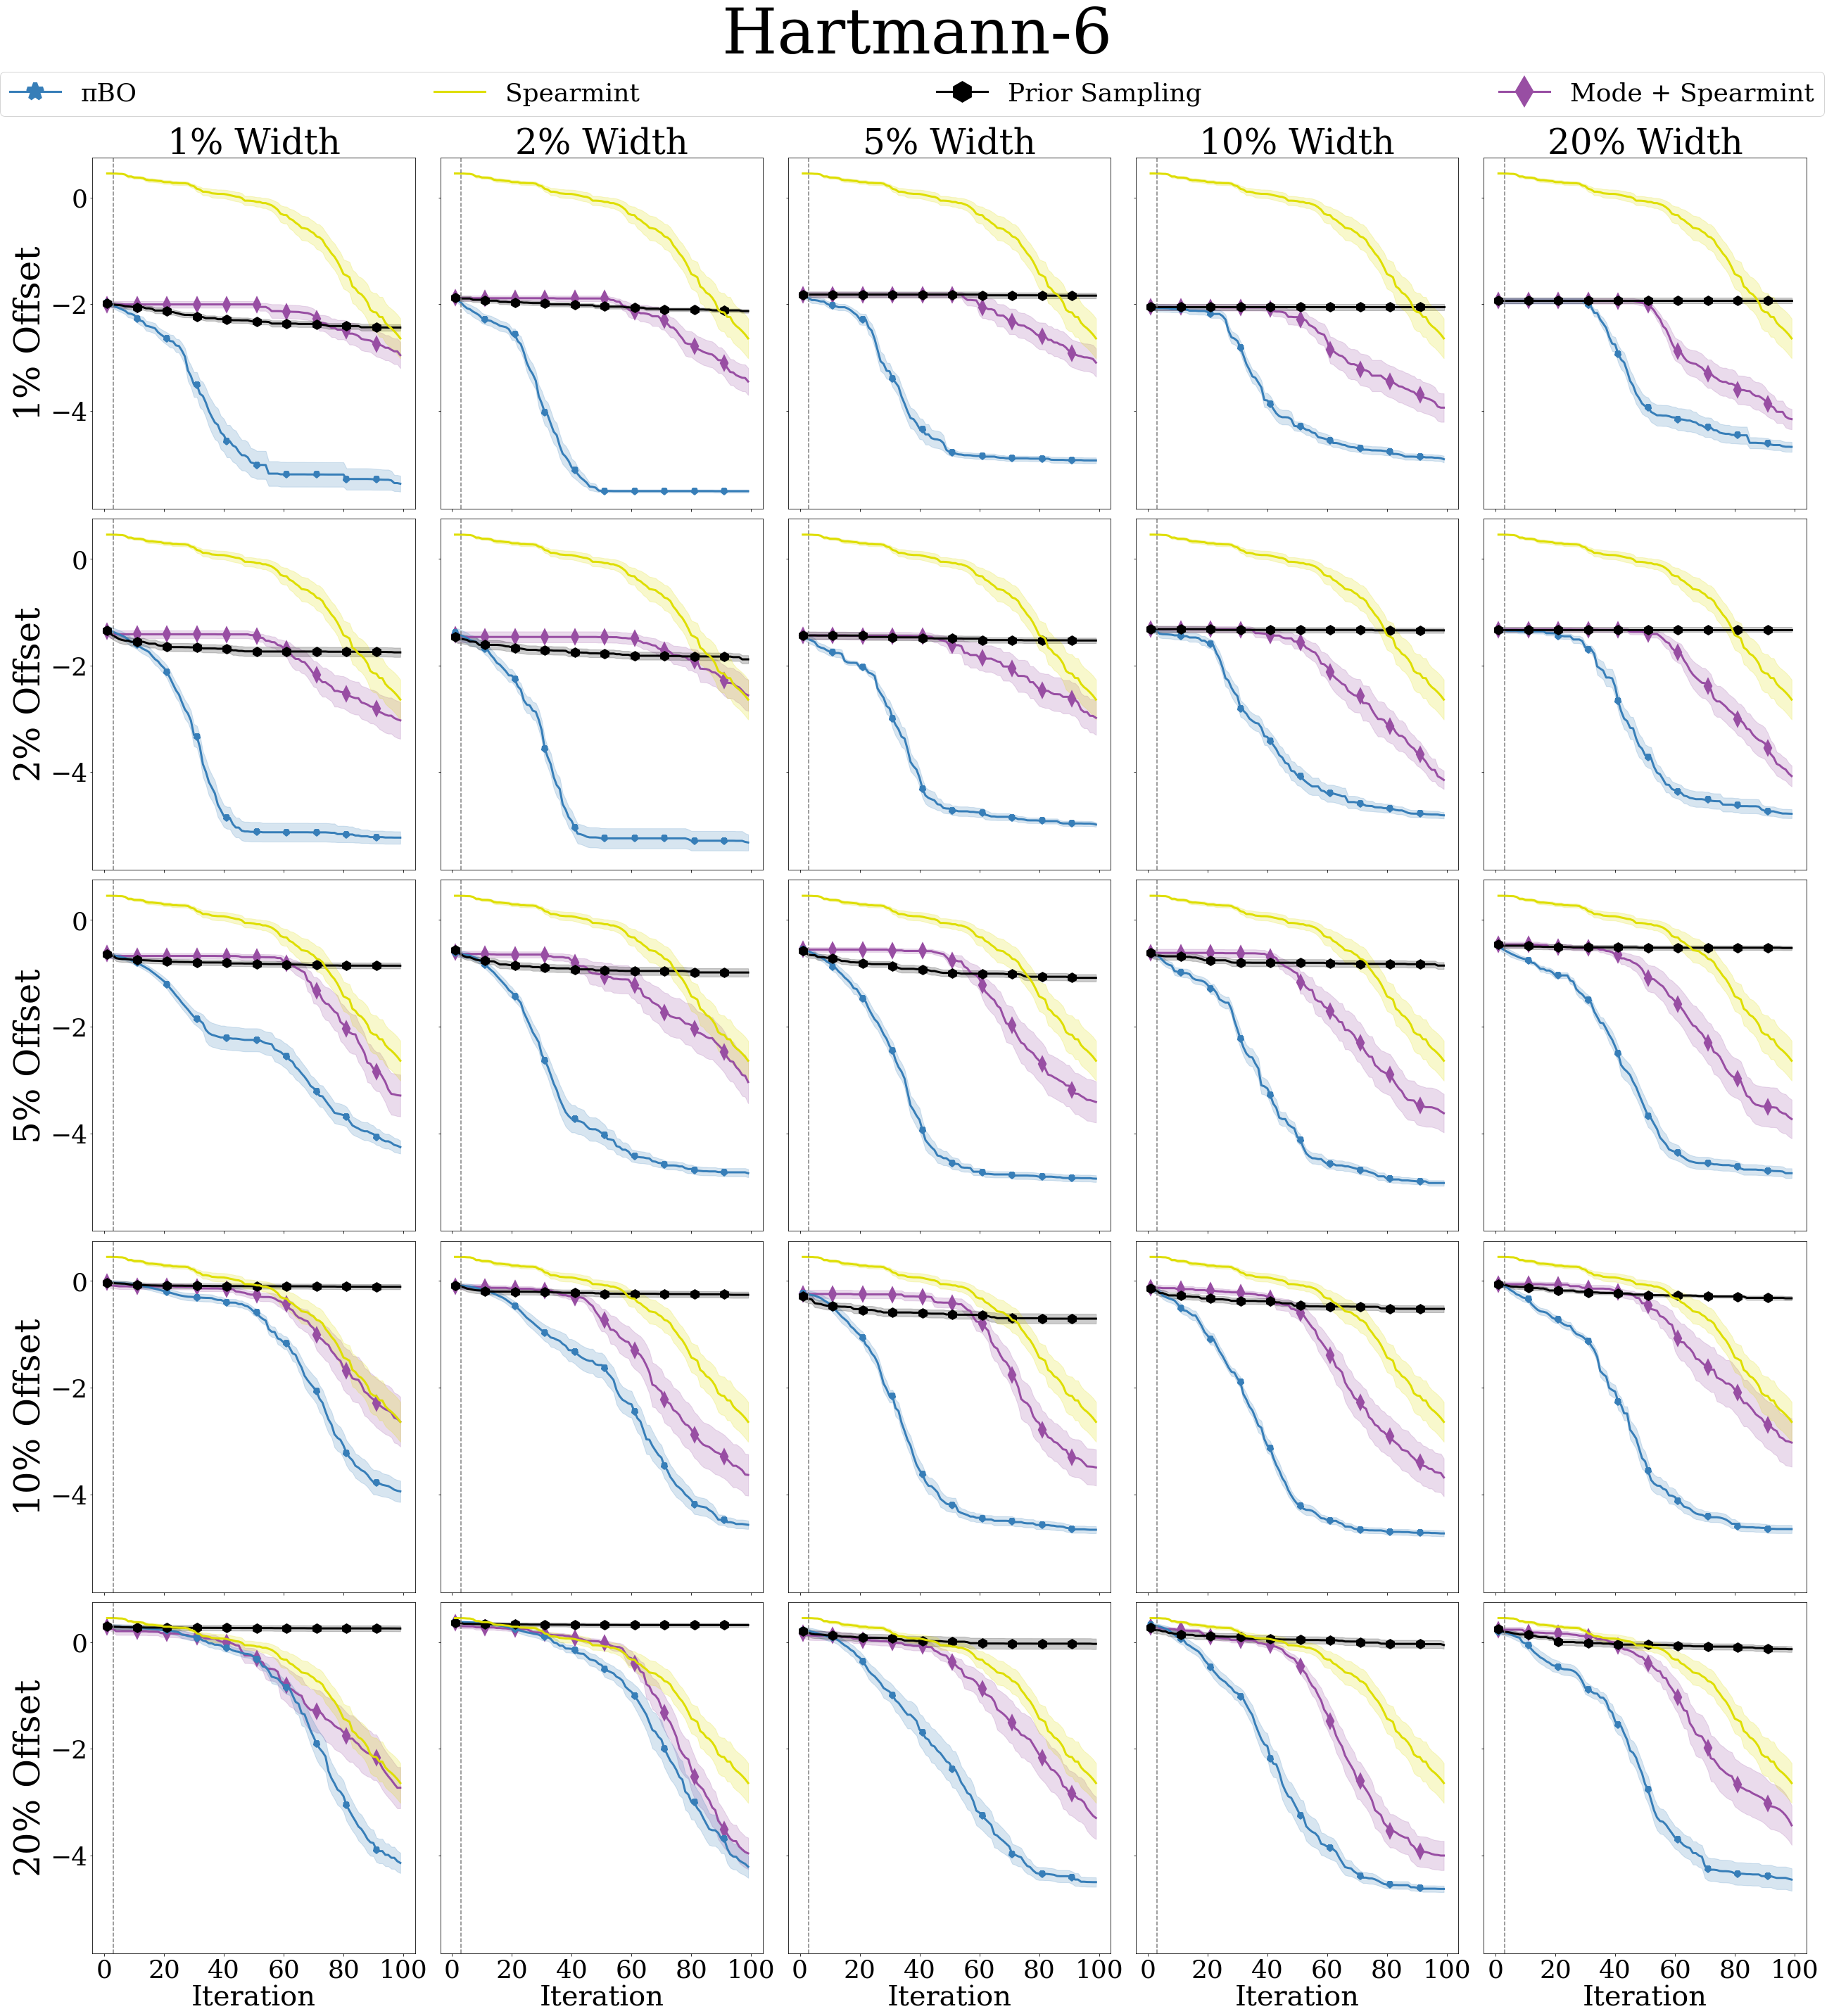
\includegraphics[width=\linewidth]{images/harmann_grid.png}
    \caption{Comparison on Hartmann-6 of priors with varying widths and offsets over the optimum on \method{}, Spearmint, Spearmint with mode initialization, and sampling from the prior. The mean and standard error of log simple regret is displayed over 100 iterations, averaged over 20 repetitions. Iteration 1 is removed for visibility purposes.}
    \label{fig:hartmann_grid}
\end{figure}
\begin{figure}
    \centering
    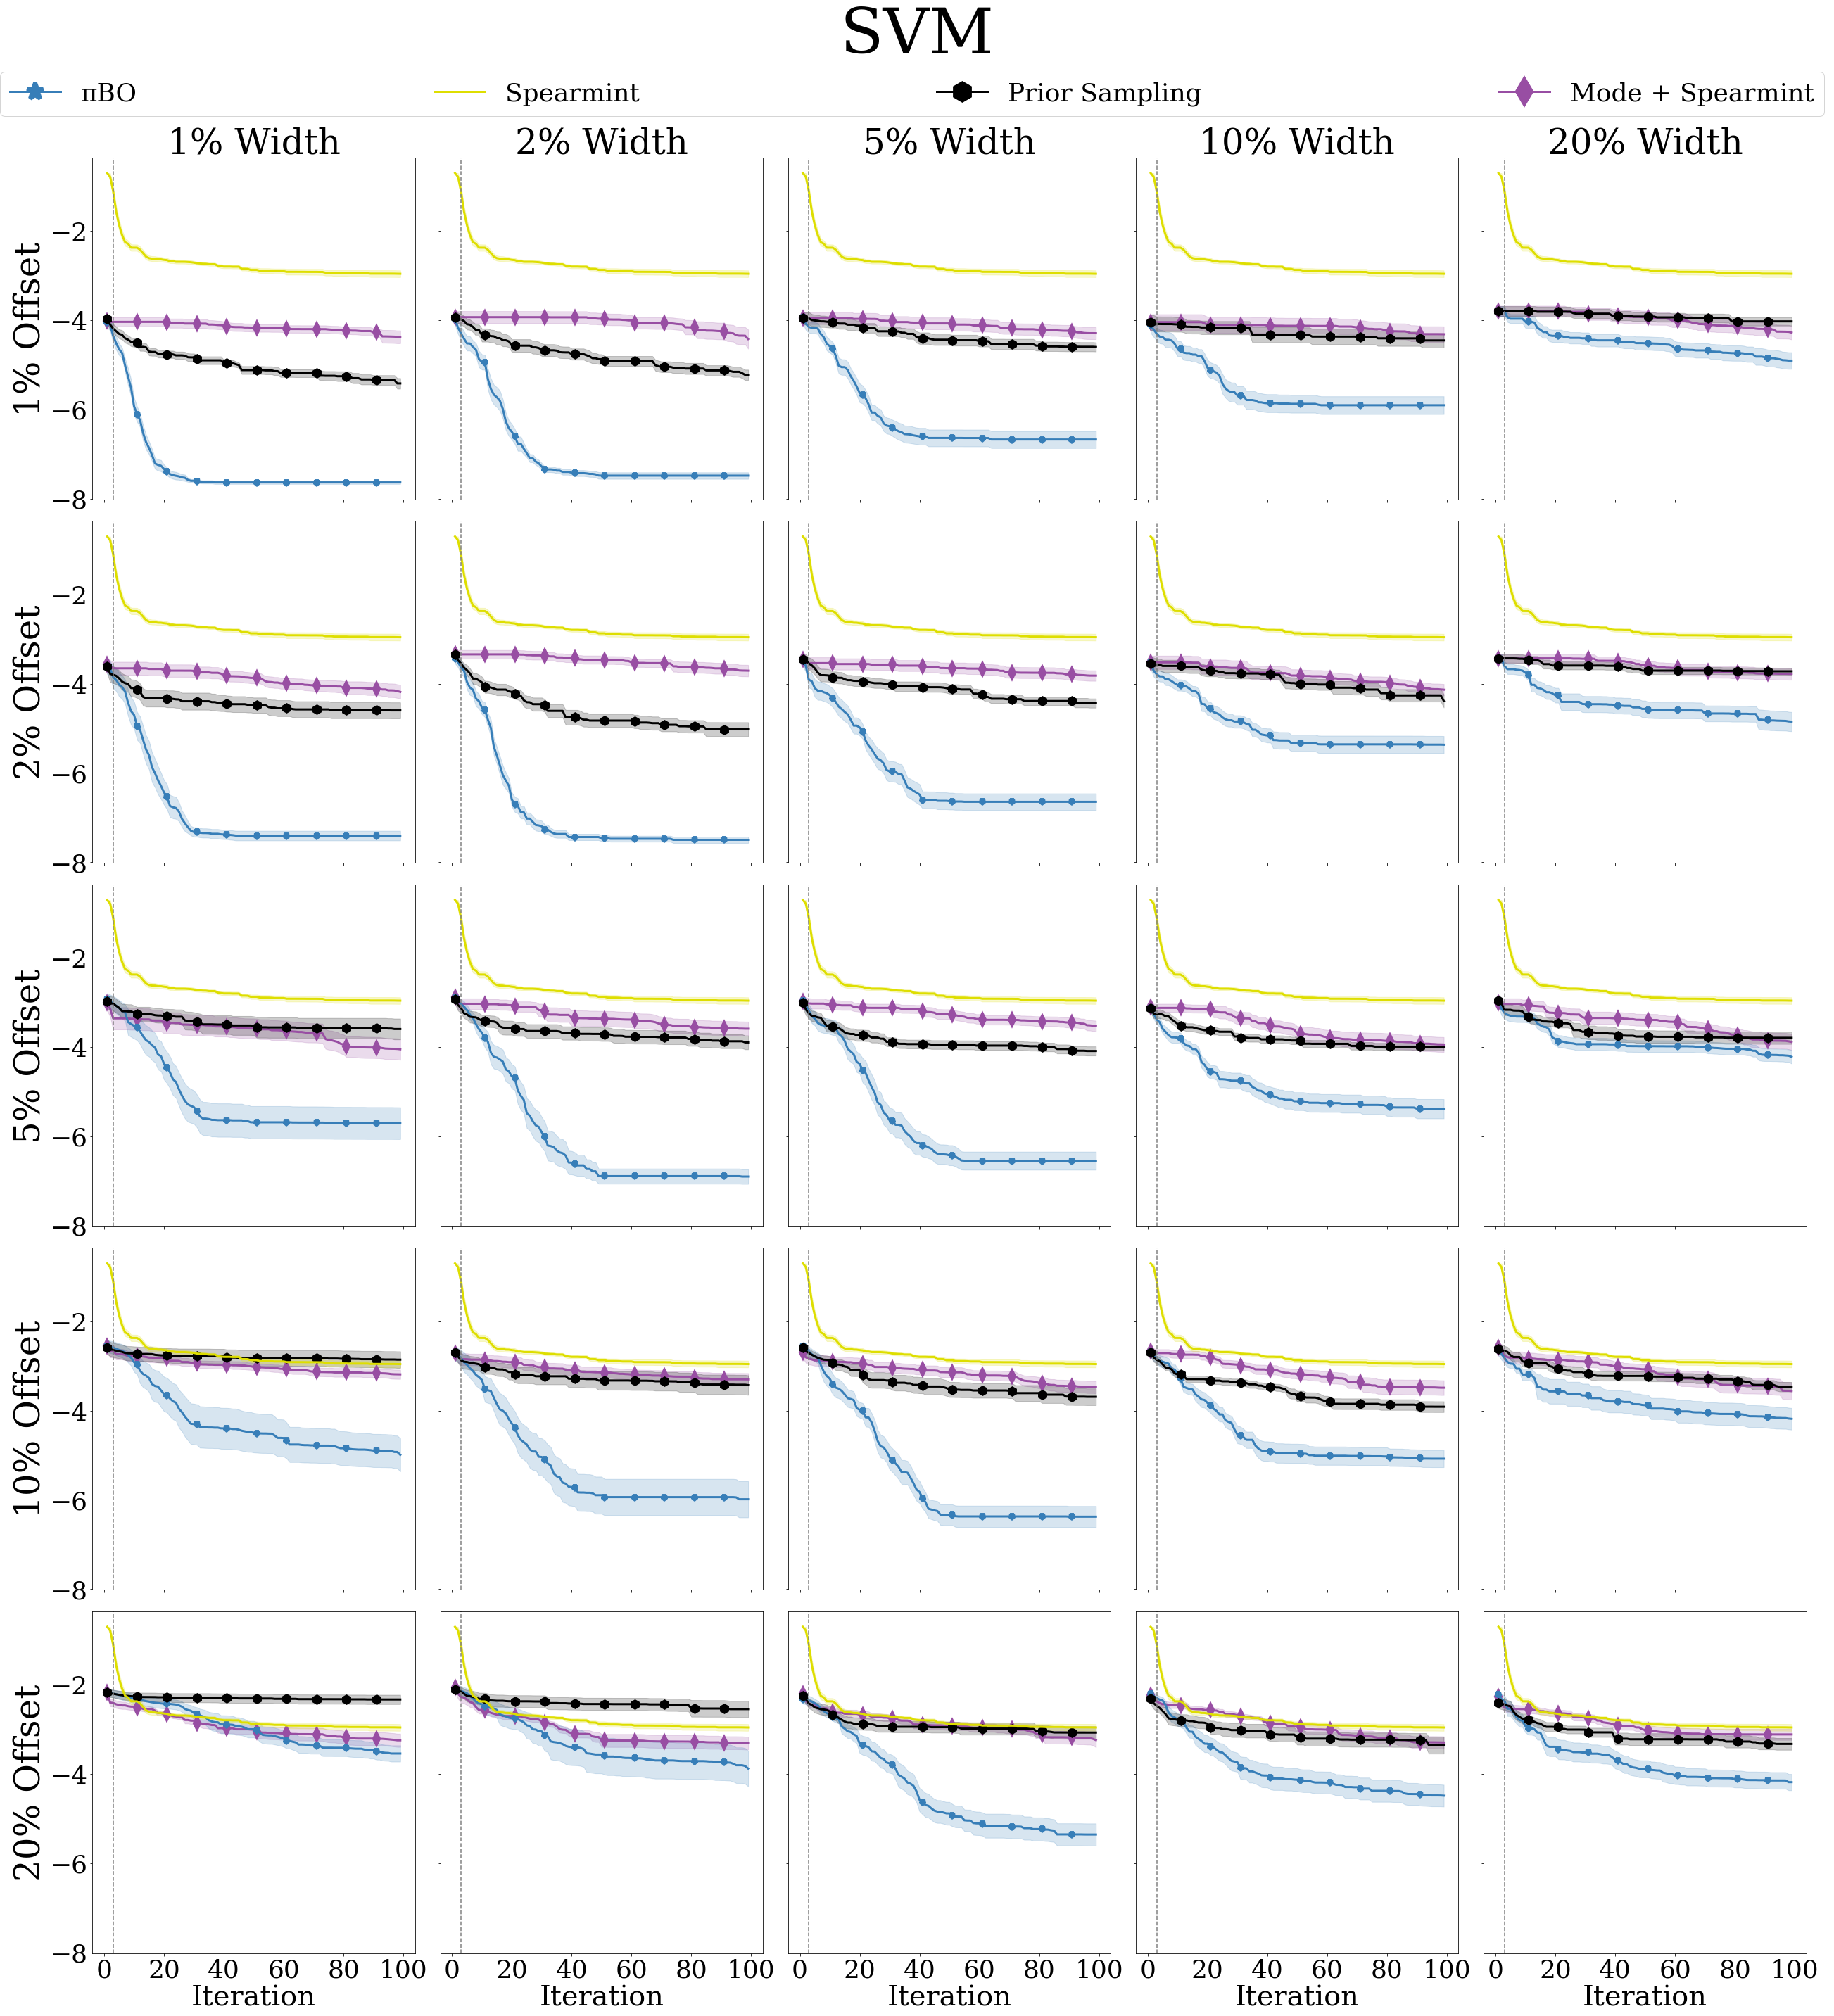
\includegraphics[width=\linewidth]{images/svm_grid.png}
    \caption{Comparison on SVM of priors with varying widths and offsets over the optimum on \method{}, Spearmint, Spearmint with mode initialization, and sampling from the prior. The mean and standard error of log simple regret is displayed over 100 iterations, averaged over 20 repetitions. Iteration 1 is removed for visibility purposes.}
    \label{fig:svm_grid}
\end{figure}
\begin{figure}
    \centering
    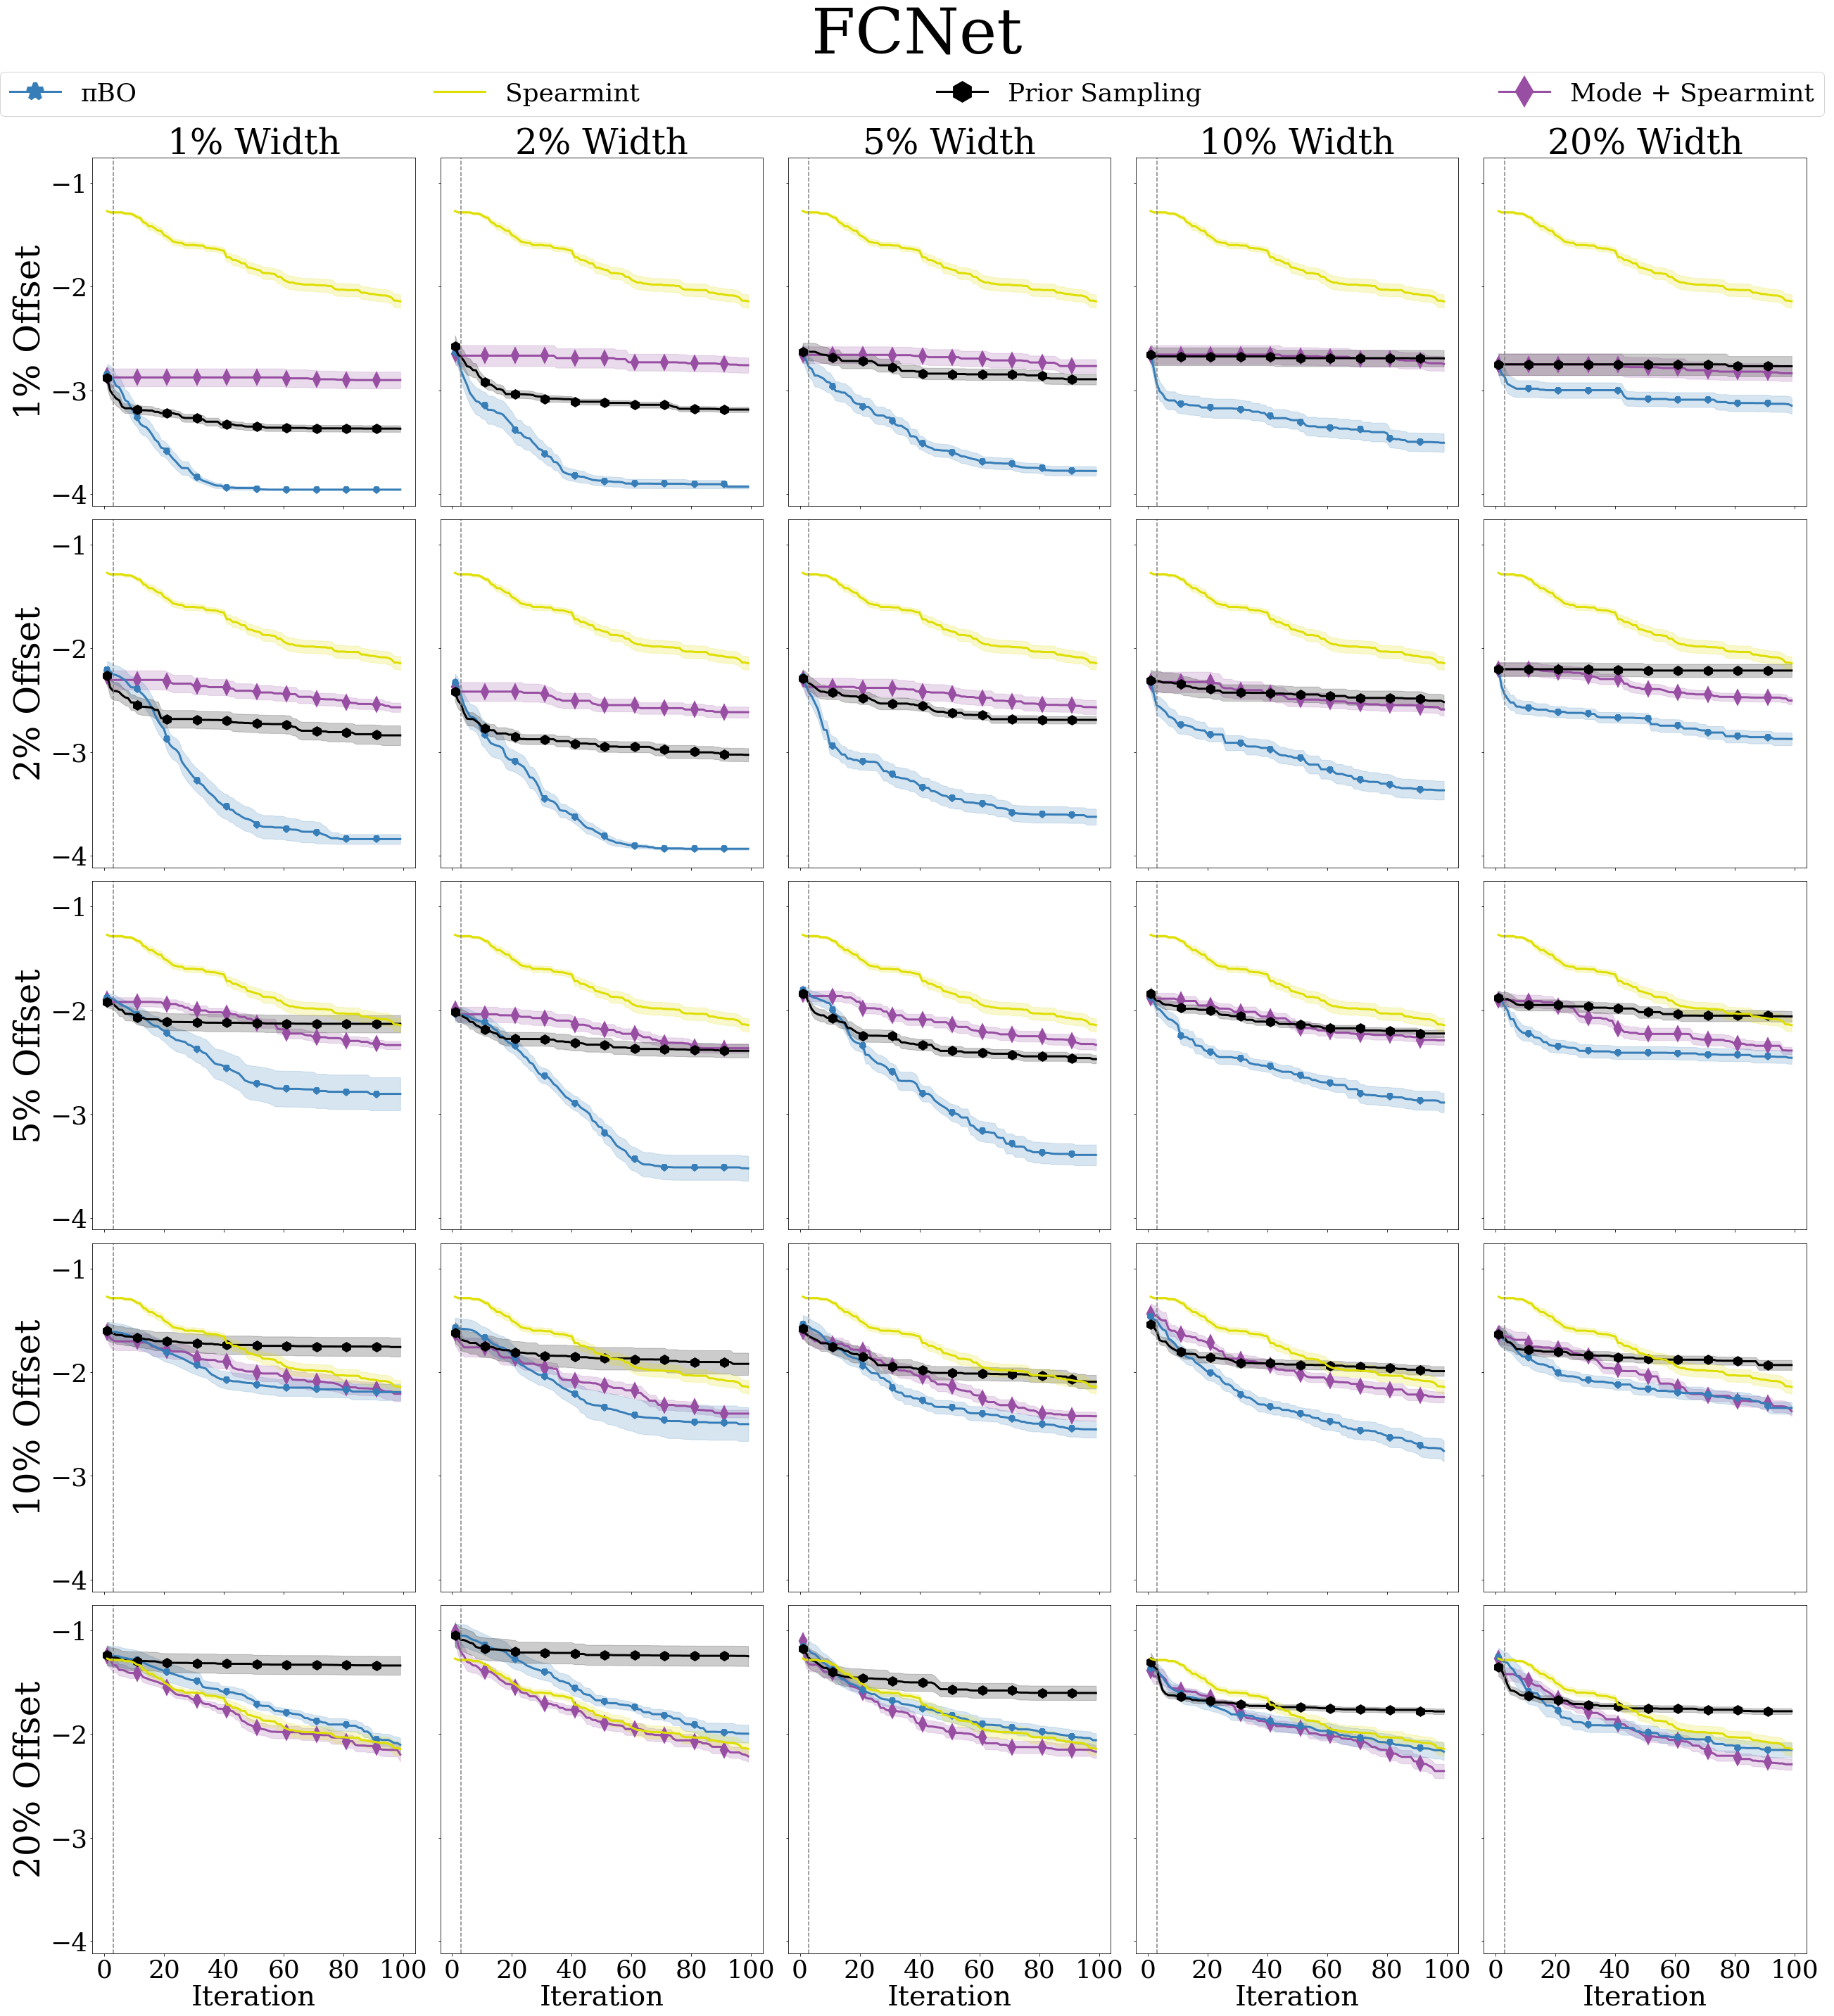
\includegraphics[width=\linewidth]{images/fcnet_grid.png}
    \caption{Comparison on FCNet of priors with varying widths and offsets over the optimum on \method{}, Spearmint, Spearmint with mode initialization, and sampling from the prior. The mean and standard error of log simple regret is displayed over 100 iterations, averaged over 20 repetitions. Iteration 1 is removed for visibility purposes.}
    \label{fig:fcnet_grid}
\end{figure}
\begin{figure}
    \centering
    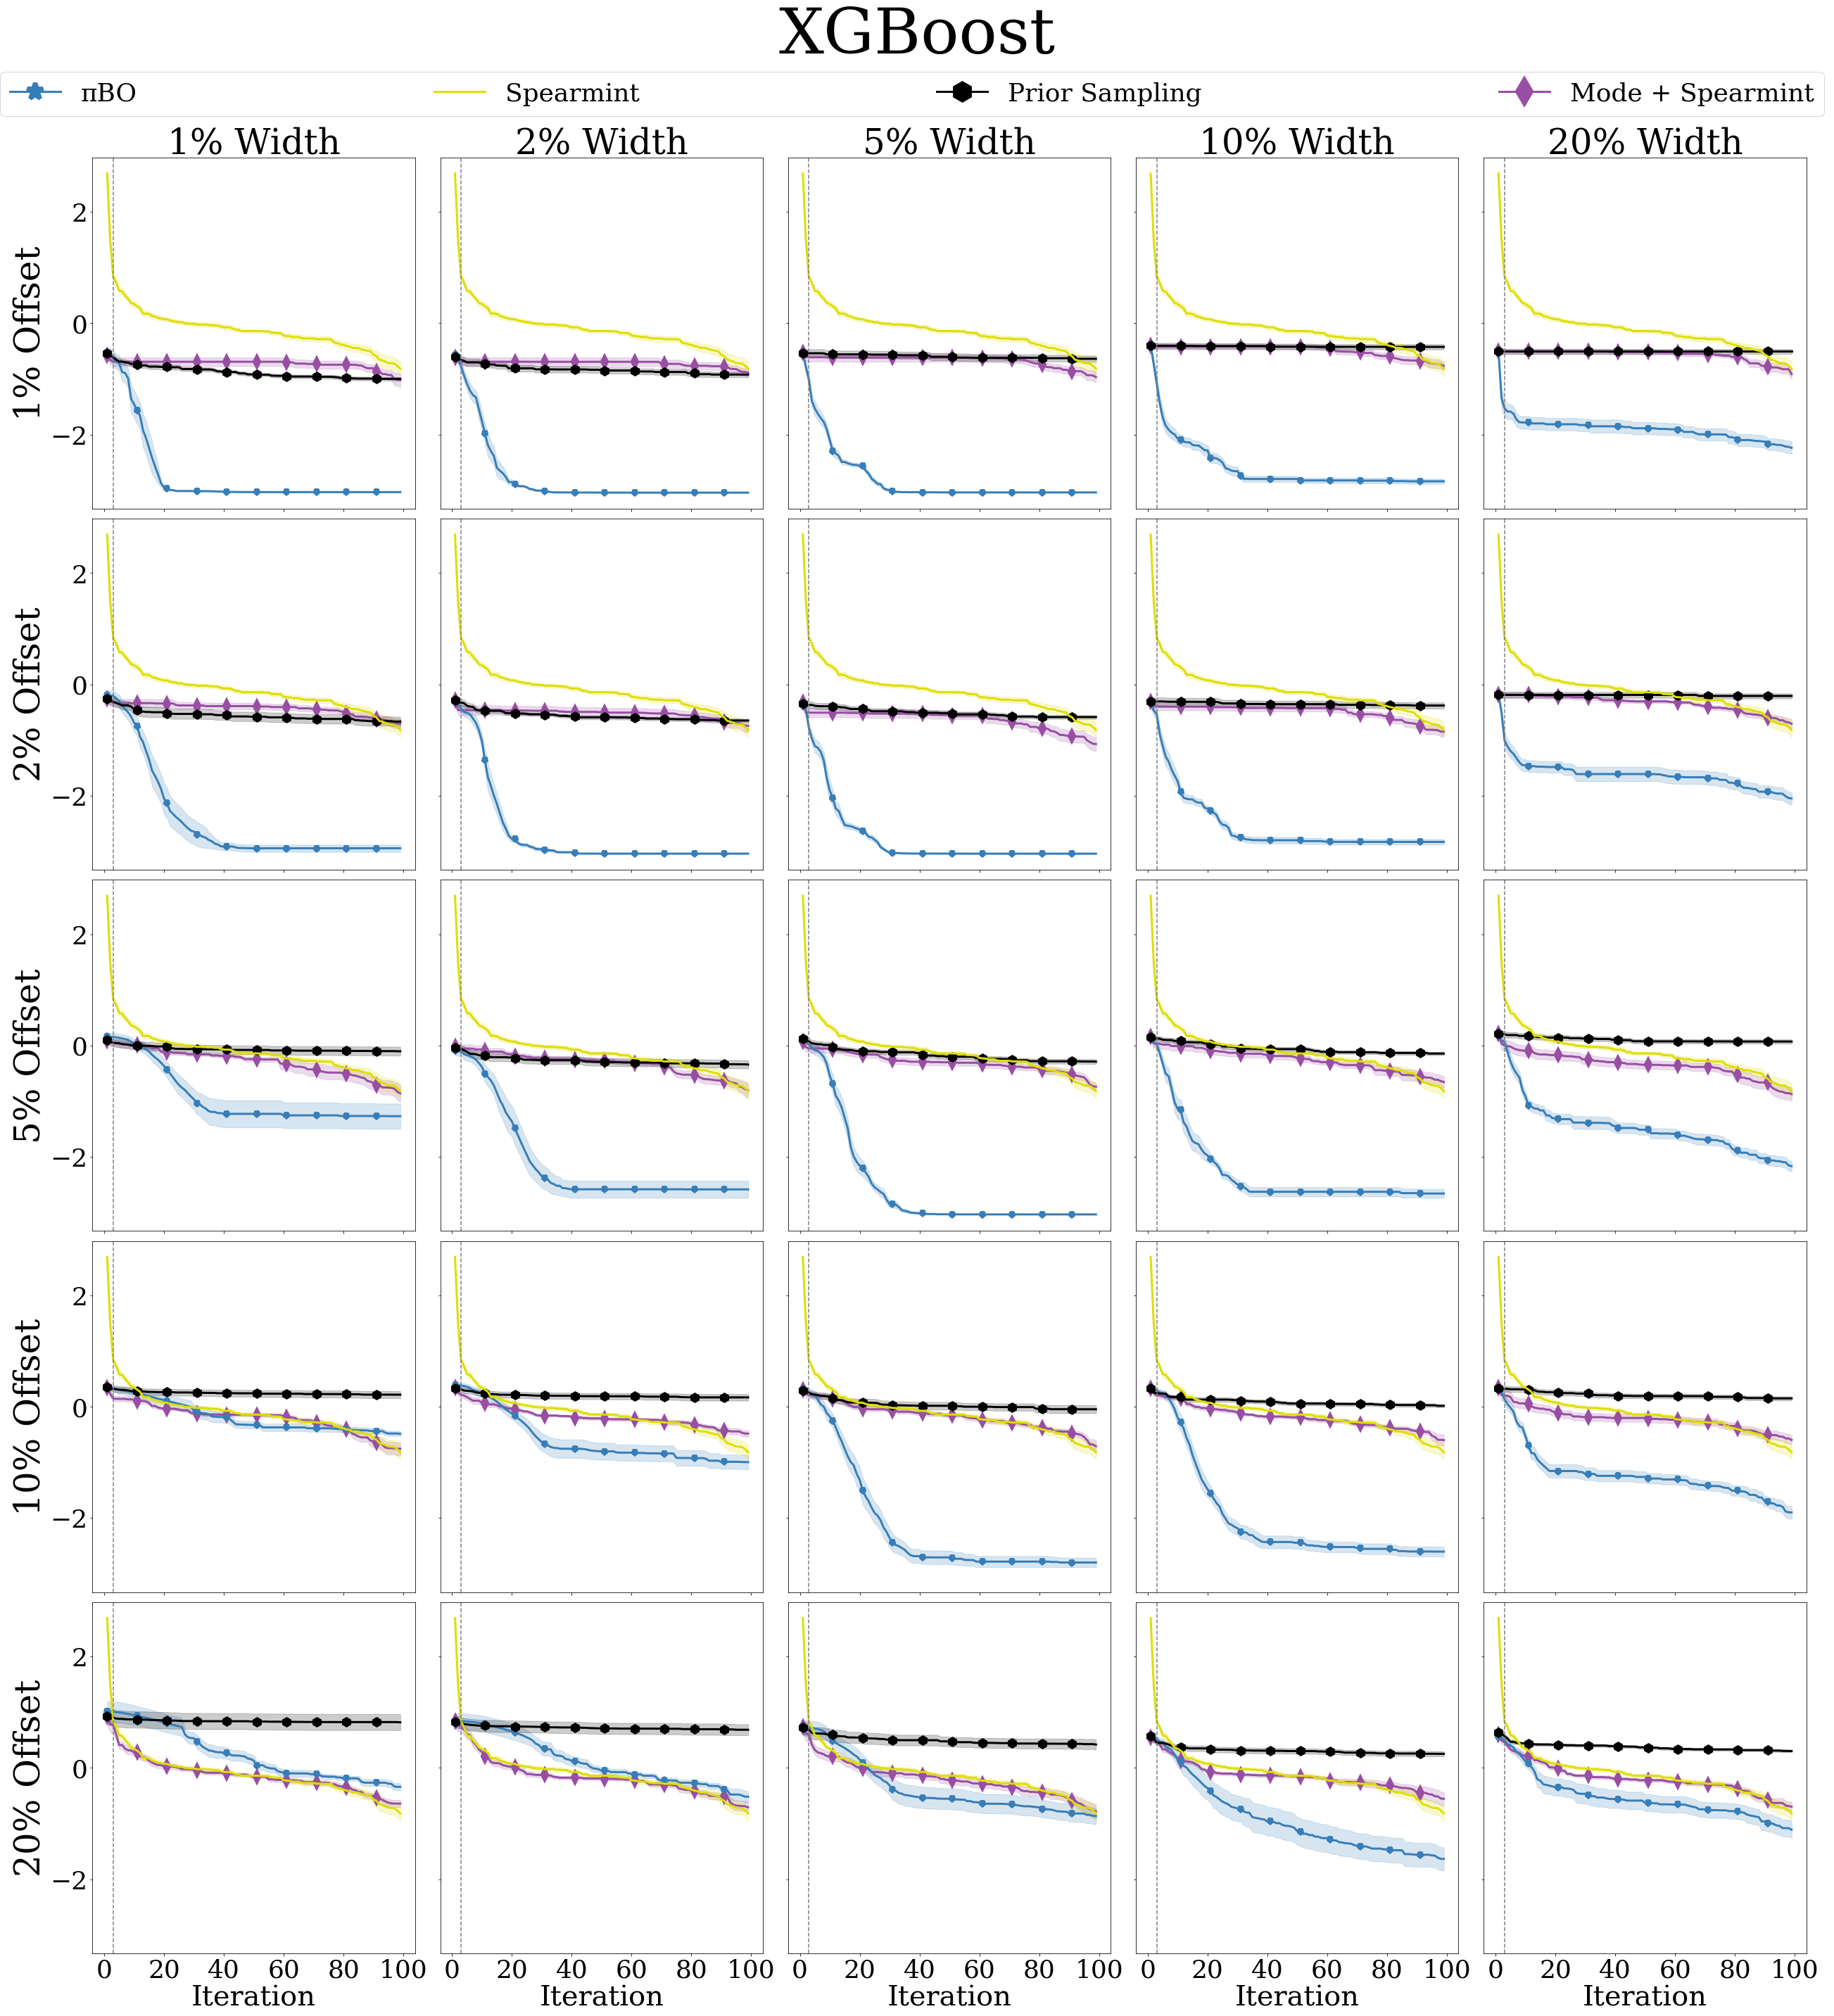
\includegraphics[width=\linewidth]{images/xgboost_grid.png}
    \caption{Comparison on XGBoost of priors with varying widths and offsets over the optimum on \method{}, Spearmint, Spearmint with mode initialization, and sampling from the prior. The mean and standard error of log simple regret is displayed over 100 iterations, averaged over 20 repetitions. Iteration 1 is removed for visibility purposes.}
    \label{fig:xgboost_grid}
\end{figure}